\documentclass[11pt]{article}

\usepackage[utf8x]{inputenc}	
\usepackage{fullpage}		
\usepackage[english]{babel}			
%\usepackage[sc]{mathpazo} %Like Palatino with extensive math support
\usepackage{fourier}

%\usepackage{ulem}
\usepackage{xcolor}						
\usepackage{amsmath,amstext,amssymb,amsfonts,amsthm,mathrsfs,chemarrow,stackrel,dsfont}   % Math packages
\usepackage{graphicx} 					
\usepackage{subcaption}					
%\usepackage{cite}	
\usepackage[authoryear,sectionbib,sort]{natbib} % Bio citation format
\linespread{1.7}
%\usepackage{titlesec}
%\titleformat{\section}[block]{\Large\bfseries\filcenter}{\thesection}{1em}{}
%\titleformat{\subsection}[block]{\Large\itshape\filcenter}{\thesubsection}{1em}{}
%\titleformat{\subsubsection}[block]{\large\itshape}{\thesubsubsection}{1em}{}
%\titleformat{\paragraph}[runin]{\itshape}{\theparagraph}{1em}{}[. ]\renewcommand{\refname}{Literature Cited}

\usepackage{titlesec}
\titleformat{\section}[block]{\Large\bfseries\filcenter}{\thesection}{1em}{}
\titleformat{\subsection}[block]{\Large\itshape\filcenter}{\thesubsection}{1em}{}
\titleformat{\subsubsection}[block]{\large\itshape}{\thesubsubsection}{1em}{}
\titleformat{\paragraph}[runin]{\itshape}{\theparagraph}{1em}{}[. ]\renewcommand{\refname}{Literature Cited}

\usepackage{enumitem}

\usepackage{microtype}
\usepackage{array}
\usepackage{booktabs}
\usepackage{makecell}

%%%%%% XX To be removed before submission!
\usepackage{lineno}
\usepackage{showlabels}

\usepackage[pdftex, breaklinks, colorlinks, citecolor=black, urlcolor=black, linkcolor=black]{hyperref} 
%\usepackage{fourier} % FD I try to avoid the default LaTeX font for non math journals
%\usepackage{FiraSans}
%\usepackage[T1]{fontenc}				

\usepackage{soul}

% Packages to comment out before submitting!
\usepackage[textsize = scriptsize, backgroundcolor = white, linecolor = black]{todonotes}
%\usepackage{showlabels}

%\numberwithin{equation}{section}
%\setlength{\parindent}{0pt}
\allowdisplaybreaks[2]

\newcolumntype{P}[1]{>{\centering\arraybackslash}m{#1}}     % Table formatting
\renewcommand{\arraystretch}{1.1}                           % Table formatting

\definecolor{darkgreen}{rgb}{0.0, 0.42, 0.24}
\definecolor{darkblue}{rgb}{0.0, 0.0, 0.55}
\definecolor{change}{rgb}{0.5,0.,0.6}

%%%%%% our commenting commands
\newcommand{\florence}[1]{\textcolor{purple}{(#1)}} % Changed red to purple
\newcommand{\francois}[1]{\textcolor{blue}{(#1)}}
\newcommand{\hildegard}[1]{\textcolor{darkgreen}{(#1)}}
\newcommand{\pete}[1]{\textcolor{orange}{(#1)}}
\newcommand{\chg}[1]{\textcolor{change}{#1}}


%%% Fix for lineno and align
\newcommand*\patchAmsMathEnvironmentForLineno[1]{%
	\expandafter\let\csname old#1\expandafter\endcsname\csname #1\endcsname
	\expandafter\let\csname oldend#1\expandafter\endcsname\csname end#1\endcsname
	\renewenvironment{#1}%
	{\linenomath\csname old#1\endcsname}%
	{\csname oldend#1\endcsname\endlinenomath}}% 
\newcommand*\patchBothAmsMathEnvironmentsForLineno[1]{%
	\patchAmsMathEnvironmentForLineno{#1}%
	\patchAmsMathEnvironmentForLineno{#1*}}%
\AtBeginDocument{%
	\patchBothAmsMathEnvironmentsForLineno{equation}%
	\patchBothAmsMathEnvironmentsForLineno{align}%
	\patchBothAmsMathEnvironmentsForLineno{flalign}%
	\patchBothAmsMathEnvironmentsForLineno{alignat}%
	\patchBothAmsMathEnvironmentsForLineno{gather}%
	\patchBothAmsMathEnvironmentsForLineno{multline}%
}
%%%


%%%APPENDIX
\usepackage[toc,page,header]{appendix}
\usepackage{minitoc}

\usepackage{chapterbib}

%%%
%opening
\title{The effect of habitat choice on evolutionary rescue in subdivided populations}
\author{Peter Czuppon$^{1,2,\ast}$, Fran\c{c}ois Blanquart$^{1,3}$, Hildegard Uecker$^{4,\dag}$,\\ Florence D\'{e}barre$^{2,\dag}$}
\date{}


\begin{document}

\doparttoc % Tell to minitoc to generate a toc for the parts
\faketableofcontents % Run a fake tableofcontents command for the partocs

% Make the "Part I" text invisible
\renewcommand \thepart{}
\renewcommand \partname{}

%\part{} % Start the document part
%\parttoc % Insert the document TOC


\maketitle

\vspace{-20pt}
\noindent $^1$ Center for Interdisciplinary Research in Biology, CNRS, Coll\`ege de France, PSL Research University, Paris, France.

\noindent $^2$ Institute of Ecology and Environmental Sciences of Paris, Sorbonne Universit\'e, UPEC, CNRS, IRD, INRA, Paris, France.

\noindent $^3$ IAME, UMR 1137, INSERM, Universit\'{e} Paris Diderot, Paris, France.

\noindent $^4$ Research Group ``Stochastic evolutionary dynamics'', Department of Evolutionary Theory, Max-Planck Institute for Evolutionary Biology, Pl\"{o}n, Germany.

\noindent $\ast$ Corresponding author; e-mail: peter.czuppon@college-de-france.fr.

\noindent $^\dag$ Equal contribution.

\noindent The authors wish to be identified to the reviewers (the manuscript is already on bioRxiv so the identities of all authors can be easily found).

\bigskip

\textit{Manuscript elements}: Figures~1-6, Table~1, Supplementary Information including figures S1-S6. All figures are to print in color.

\bigskip

\textit{Keywords}: evolutionary rescue, local adaptation, source-sink dynamics, dispersal, gene flow, habitat choice, density-dependent dispersal.

\bigskip

\textit{Manuscript type}: Article. %Or e-article, note, e-note, natural history miscellany, e-natural history miscellany, comment, reply, invited symposium, or countdown to 150.

\newpage

\linenumbers{}
\modulolinenumbers[2]
\part{}

\begin{abstract}
    \noindent \textbf{Abstract} Evolutionary rescue is the process by which a declining population successfully adapts genetically\footnote{\francois{remove genetically}\florence{ok to remove}} to avoid extinction. In a structured environment that deteriorates patch by patch, dispersal can substantially alter the chances of evolutionary rescue of a \linelabel{R2-1}\chg{population whose wild type is} not viable in deteriorated patches. Here, we investigate the effect of different dispersal schemes and intensities on the probability of successful establishment of a mutant population adapted to the deteriorated environment. \linelabel{R1-2}\chg{We assume that local fitness is determined by a single haploid locus\florence{ and that d}\st{. D}ispersal is genotype-dependent\st{ and linked to the adaptive trait, i.e. dispersal does not evolve by itself}\footnote{\florence{[otherwise it sounds like $m$ is changing...] [need to add that it's the bias that is changing, not the probability to emigrate]}}. In this scenario, we }find that the probability of evolutionary rescue can undergo up to three phases when increasing the rate of dispersal\footnote{\florence{since you specify ``at low disp'', ``at intermediate disp'' etc., you can remove ``when increasing the rate of dispersal'' to save words}}: (i) at low dispersal rates, the probability of establishment of a mutant population increases; (ii) at intermediate dispersal rates, the establishment probability decreases; (iii) at large dispersal rates, the population homogenizes, \florence{, which either promotes or suppresses}\footnote{\florence{old version: either promoting or suppressing}} the process of evolutionary rescue, depending on the fitness difference between the mutant and the wild type. Our results show that habitat choice\footnote{\florence{up to now, the reader does not know this is about habitat choice (``schemes'' is not precise enough}}, when compared to \chg{unbiased} dispersal, impedes successful adaptation when the mutant has the same habitat preference as the wild type, but promotes adaptation when the mutant mainly immigrates into patches where it has a growth advantage over the wild type.
\end{abstract}

%\textit{Keywords:} evolutionary rescue, local adaptation, source-sink dynamics, dispersal, gene flow, habitat choice, density-dependent dispersal

%%%%%%%%%%%%%%%%%%%%%%%%%%%%%%%%%%%%%%%%%%%%%%%%%%%%%%%%%%%%%%%%%%%
%%%%%%%%%%%%%%%%% INTRODUCTION %%%%%%%%%%%%%%%%%%%%%%%%%%%%%%%%%%%%
%%%%%%%%%%%%%%%%%%%%%%%%%%%%%%%%%%%%%%%%%%%%%%%%%%%%%%%%%%%%%%%%%%%
\newpage

\section*{Introduction}

%%%%%%%%%%%%%%%%%%%%%%%%%%%%%%%%%%%%%%%%%%%%%%%%%
% Evol rescue and empirical evidence %%%%%%%%%%%%
%%%%%%%%%%%%%%%%%%%%%%%%%%%%%%%%%%%%%%%%%%%%%%%%%
Current anthropogenic environmental changes such as deforestation, soil and water contamination or rising temperatures, contribute to the decline of the populations of many species, that might eventually go extinct \citep{bellard_2012, diniz_2019}. Pests and pathogens experience similarly strong selective pressures as a result of increased consumption of antibiotics and use of pesticides \citep{ramsayer_2013, kreiner_2018}. 
The process of genetic\footnote{\florence{rescue by plasticity as well}} adaptation that saves populations from extinction is termed evolutionary rescue. This \linelabel{R1-3}\chg{process is characterized by an initial population decline (that would result in population extinction) followed by recovery due to the establishment of adapted genotypes, } \florence{classically} resulting in a U-shaped demographic trajectory over time~\citep{gomulkiewicz_1995}.
In recent years, empirical examples of evolutionary rescue have accumulated \citep[as reviewed by ][]{alexander_2014,carlson_2014,bell_2017}. Laboratory experiments have provided direct evidence of evolutionary rescue \linelabel{R1-4} \citep[e.g.][]{bell_2009, agashe_2011, lachapelle_2012, lindsey_2013, stelkens_2014}. In the wild, however, demographic and genotypic data are rarely monitored together at the same time, which impedes direct observation of evolutionary rescue. Still, evolutionary rescue has been suggested as a mechanism that has saved a few wild populations from extinction \citep[e.g.][]{vanderwal_2012, digiallonardo_2015, gignoux_2018}. 


%% Genetic setting

\florence{[Need a paragraph on the genetic makeup. We are not explaining this at all at the moment and this is lacking] Rescue can occur through plasticity (refs Chevin? \footnote{https://royalsocietypublishing.org/doi/full/10.1098/rspb.2016.1690 , https://royalsocietypublishing.org/doi/abs/10.1098/rstb.2012.0089 and/or https://onlinelibrary.wiley.com/doi/full/10.1111/j.1558-5646.2009.00875.x}) or genetic adaptation (refs). The traits involves can be continuous (ref) or discrete (ref). In this work, we consider genetic adaptation mediated by discrete traits. Specifically, we consider that a single mutation can prevent extinction, and...}

%%%%%%%%%%%%%%%%%%%%%%%%%%%%%%%%%%%%%%%%%%%%%%%%%
% Evol rescue and dispersal %%%%%%%%%%%%%%%%%%%%%
%%%%%%%%%%%%%%%%%%%%%%%%%%%%%%%%%%%%%%%%%%%%%%%%%
In mathematical models, evolutionary rescue is often studied in a spatially homogeneous situation where the whole population experiences a sudden decrease in habitat quality. In this setting, a large number of theoretical results have been established, for example on the effects of recombination \citep{uecker_2015} and 
horizontal gene transfer \citep{tazzyman_2014}, 
reproduction mechanisms \citep{glemin_2013,uecker_2017}, intra- and interspecific competition \citep{osmond_2013}, predation pressure \linelabel{R1-5}\citep{yamamichi_2015}, 
bottlenecks \citep{martin_2013}, 
different genetic pathways \citep{osmond_2019}, and the context-dependent fitness effects of mutations \citep{anciaux_2018}. \chg{In contrast to these abrupt change scenarios, evolutionary rescue can also be studied in a gradually changing environment \citep[e.g.][]{osmond_2017}}\footnote{\pete{Does anybody know other references?} \hildegard{What about Lynch et al. 1991. Adaptive and  demographic responses of plankton populations to environmental change. Limnology and Oceanography 36:1301--1312., B{\"u}rger and Lynch 1995. Evolution and extinction in a changing environment: a quantitative genetic analysis. Evolution 49:151--163 and Lande and Shannon 1996. The role of  genetic  variation  in adaptation and population persistence in a changing environment. Evolution 50:434--437? But please check; it's a long time that I read those...}}. 
Such gradual changes can in particular occur in fragmented environments.

In fragmented environments, habitat deterioration is not necessarily synchronized across patches: there can be a transient spatially heterogeneous environment consisting of a mosaic of old and of degraded habitat patches, until eventually the whole environment has deteriorated. If individuals that populate different patches are able to move between those, the effect of dispersal on evolutionary rescue needs to be taken into account \citep{uecker_2014, tomasini_2019}. \linelabel{R1-1}\chg{The intensity of dispersal among patches tunes how abruptly environmental change is experienced. With very low dispersal, patches are essentially isolated from each other, and each patch undergoes an abrupt change independently of the other patches. With higher dispersal, asynchronous deterioration among patches is experienced as a more gradual change overall.}
Experiments that study the effect of dispersal on evolutionary rescue are rare, but, for instance, \citet{bell_2011} found that \linelabel{R1-6} dispersal can increase the likelihood of successful genetic adaptation. 

%%%%%%%%%%%%%%%%%%%%%%%%%%%%%%%%%%%%%%%%%%%%%%%%%
% Adaptation and dispersal %%%%%%%%%%%%%%%%%%%%%%
%%%%%%%%%%%%%%%%%%%%%%%%%%%%%%%%%%%%%%%%%%%%%%%%%
The transient mosaic of degraded and non-degraded patches that results from asynchronous degradation in a fragmented habitat is similar to the setting of models of source-sink dynamics. These models represent a spatially heterogeneous environment, constant in time, in which wild-type populations in unfavorable habitats can only be maintained thanks to recurrent immigration from favorable habitats. 
Experimental and theoretical studies have found that \linelabel{R2-3}\chg{increasing} dispersal can have a positive or a negative effect on genetic adaptation in a heterogeneous environment (see e.g., for studies on discrete traits, \florence{[refocus the citations with papers on discrete traits; otherwise there are too many possible citations -- it's fine to do so given that we now explicitly say the paper is focused on discrete traits]}\citet{holt_1997,gomulkiewicz_1999} for positive; \citet{storfer_1998,garcia_1997,kirkpatrick_1997,fedorka_2012} for negative; and \linelabel{R1-7}\chg{\citet{kawecki_2000, gallet_2018}} for both effects).
%Reason for different results: (i) demography or not (Kawecki); (ii) selection strength (Gallet), (iii) selection strength (Ronce)

%%% DISPERSAL, biased or not
In theoretical studies of local adaptation and evolutionary rescue, dispersal is typically assumed to be \chg{unbiased}, i.e. dispersing individuals are distributed uniformly among patches. Only few investigations in the context of local adaptation in source-sink systems have taken into account non-\chg{uniform} dispersal patterns \citep[e.g.][]{kawecki_1995,holt_1996,kawecki_2002,amarasekare_2004}. This analytical focus on \chg{unbiased} dispersal is in stark contrast to dispersal schemes observed in nature \citep[][]{edelaar_2008,clobert_2009,edelaar_2012}. 

%%%%%%%%%%%%%%%%%%%%%%%%%%%%%%%%%%%%%%%%%%%%%%%%%
% Empirical examples for non-random dispersal %%%
%%%%%%%%%%%%%%%%%%%%%%%%%%%%%%%%%%%%%%%%%%%%%%%%%
One of the best documented modes of non-\chg{uniform} dispersal is density-dependent dispersal. Density dependence can be positive or negative: either individuals prefer to settle or stay in large groups (positive density-dependence), or they choose to remain in or move to less populated regions (negative density-dependence). Density-dependent dispersal, of either form, is ubiquitously found in nature and has been reported in many species across the tree of life, including insects \citep{endriss_2019}, spiders \citep{meester2010}, amphibians \citep{gautier_2006}, birds \citep{wilson_2017}, fishes \citep{turgeon_2012}, and mammals~\citep{stoen_2006}.

Another well-established dispersal scheme is a type of habitat choice, whereby individuals tend to immigrate into habitats they are best adapted to. This mechanism has for example been reported in lizards \citep{bestion_2015}, birds \citep{dreiss_2011,benkman_2017}, fishes \citep{bolnick_2009}, worms \citep{mathieu_2010}, and ciliates \citep{jacob_2017,jacob_2018}. 

\linelabel{R1-8} Dispersal biases can affect the different steps of dispersal (the probability to emigrate, the vagrant stage, and immigration \citep{bowler_2005,ronce_2007}). In this work, we focus on effects on the immigration step. 

%%%%%%%%%%%%%%%%%%%%%%%%%%%%%%%%%%%%%%%%%%%%%%%%%
% What do we do? %%%%%%%%%%%%%%%%%%%%%%%%%%%%%%%%
%%%%%%%%%%%%%%%%%%%%%%%%%%%%%%%%%%%%%%%%%%%%%%%%%
We model an environment that consists of various patches with one of two possible habitats: the `old' habitat, in which both \linelabel{R1-9-1}\chg{types, wild type and mutant, have a positive growth rate}, and the `new' habitat, where in the absence of immigration the wild-type population will eventually go extinct. We study four biologically motivated dispersal schemes, which correspond to the four combinations of biases towards old vs.\ new patches for wild type and mutants, and we compare these dispersal schemes to \chg{unbiased} dispersal. Our analysis is carried out step-wise. We first consider a temporally constant but spatially heterogeneous environment with two (`old' and `new') patch types. In this setting, we first study the probability of establishment of a single mutant, assuming there are no further mutations between types. We then relax the assumption of no further mutations, and compute a probability of adaptation, i.e. of establishment of the mutant lineage\footnote{\florence{not sure about this defn, please check}}. Finally, we let habitat degradation proceed, assuming that patches, one after \chg{another}, deteriorate over time until all locations contain the new habitat. Using the previous results, we approximate a probability of evolutionary rescue, i.e.\ that a mutation appears, establishes, thereby allowing the population to persist in spite of environmental degradation. We find that dispersal biases affect the probabilities of establishment and of evolutionary rescue, because it directly affects the local growth rates. 

%%%%%%%%%%%%%%%%%%%%%%%%%%%%%%%%%%%%%%%%%%%%%%%%%%%%%%%%%%%%%%%%%%%
%%%%%%%%%%%%%%%%% MODEL %%%%%%%%%%%%%%%%%%%%%%%%%%%%%%%%%%%%%%%%%%%
%%%%%%%%%%%%%%%%%%%%%%%%%%%%%%%%%%%%%%%%%%%%%%%%%%%%%%%%%%%%%%%%%%%
\section*{Model and methods}

\subsection*{Main assumptions and life-cycle}
%%%%%%%%%%%%%%%%%%%%%%%%%%
% General description %%%%
%%%%%%%%%%%%%%%%%%%%%%%%%%
We consider a spatially structured environment consisting of $M$ patches all connected to each other. The habitat of a patch is either in the \textit{old} or in the \textit{new} state, corresponding to habitat quality before and after environmental deterioration, respectively. One after \chg{another} every $\tau$ generations, the habitat of a patch deteriorates, from old to new state, the transition being irreversible. Initially ($t<0$), all patches are of the old-habitat type. At time $t=0$, the first patch deteriorates. After $(M-1)\tau$ generations, all patches are of the new-habitat type. We denote the time-dependent frequency of old-habitat patches by $f_{\text{old}}$. It equals $1$ before the first environmental change takes place ($t<0$), and decreases by $1/M$ after each environmental deterioration event, until it eventually hits~$0$, when all patches have undergone the environmental change. This setting corresponds to the one analyzed by \citet{uecker_2014}, and more recently by \citet{tomasini_2019} in the special case of just two patches\footnote{\florence{what about carrying capacities in these papers?}}. The maximum numbers of individuals that can live in a patch of a given habitat type, i.e.\ the carrying capacities, are denoted $K_{\text{old}}$ and $K_{\text{new}}$ for old- and new-habitat patches respectively; $K_{\text{old}}$ and $K_{\text{new}}$ may differ.

The population living in this environment consists of asexually reproducing, haploid individuals; generations are discrete and non-overlapping. There are two possible types of individuals, wild types and mutants. The individuals go through the following life-cycle: \begin{enumerate}[label = (\roman*)]
	\item Dispersal: individuals may move between patches. Further details about this step are given below.
	\item Reproduction: individuals reproduce within patches. \linelabel{R2-7}The number of offspring produced by an individual of type $i$ in habitat $k$ (before density regulation, if any), i.e.\ its fecundity, is drawn in a Poisson distribution of expectation $\omega_i^k$. Having fewer than $1$ offspring in expectation means that the local subpopulation will get extinct in the absence of immigration, because the deaths of the parents at each generation are not compensated by enough births on average. On the contrary, the local population is viable if the expected fecundity is greater than $1$. We assume that wild-type and mutant populations are viable in old-habitat patches, and that the mutant's expected fecundity there is lower than the wild type's: $1 \leq \omega^{\text{old}}_m < \omega^{\text{old}}_w$ \footnote{\florence{In the table, it is $0 \leq $, yet the populations are supposed to be viable}}. In new-habitat patches, a wild-type population will eventually go extinct, while a mutant one would persist, hence the term ``rescue mutant'': $\omega^{\text{new}}_w < 1 < \omega^{\text{new}}_m$. 
	All parents die at the end of this step.
	\item \linelabel{R2-9} Mutation: wild-type offspring mutate to the rescue mutant type with probability $\theta$ (back mutations from the mutant to the wild type are neglected).
	\item \linelabel{R2-8}Regulation: if the number of offspring produced locally exceeds the local carrying capacity $K_k$ (where $k$ refers to the habitat type, old or new), the population size is down-regulated to the $K_k$: individuals are randomly removed until the local population size is equal to $K_k$. One mutant offspring has the same chance of being removed as one wild-type offspring: \linelabel{AE-3} we assume that wild-type and mutant individuals are competitively equivalent. If the number of offspring is below the carrying capacity, the regulation step is ignored. We call ``successful offspring'' offspring that survive the density regulation step, and become adults at the next generation. 
	At the end of this step, all offspring become adults, and a new cycle then begins.
\end{enumerate}


%%%%%%%%%%%%%%%%%%%%%%%%%%
% Dispersal mechanisms %%%
%%%%%%%%%%%%%%%%%%%%%%%%%%
\subsection*{Dispersal mechanisms}

We split the dispersal step into emigration and immigration. Emigration is unbiased: all individuals have the same probability $m$ of leaving the patch they were born in. We assumed that dispersal biases affect the immigration step. 
We denote by $\pi_{i}$ the bias for immigration to an old-habitat patch, where the index $i$ refers to the type of the dispersing individual ($w$ for wild type, $m$ for mutant). When $\pi_i<0$, individuals of type $i$ are relatively more likely to settle in new-habitat patches than in old-habitat patches; conversely, their bias is towards old-habitat patches when $\pi_i>0$. The case $\pi_i=0$ corresponds to unbiased dispersal. 
For simplicity, we assume that dispersal is cost-free. While local population sizes may be affected by dispersal, the global size of the metapopulation remains the same before and after dispersal. \linelabel{R1-18}\linelabel{R2-14} Note that our methods can readily be applied to costly dispersal (including to costs that differ among wild-type and mutant individuals), and also to type- and habitat-dependent emigration probabilities. 

The probability that an individual of type $i$ migrates from a patch of any habitat type into a patch of the new-habitat type is\florence{TODO change into simple bias (remove m)}
%
\begin{equation}\label{eq:dispersal}
\begin{aligned}
m_i^{\text{new}} &= m\, \frac{1-f_{\text{old}}}{1-f_{\text{old}}+\chg{e^{\pi_i}} f_{\text{old}}} = 1-m_i^{\text{old}},\\
\end{aligned}
\end{equation}
\florence{there seems to be a problem with the second equation, should be $m -$ no? }
where, as defined above, $f_{\text{old}}$ is the frequency of old-habitat patches and $\pi_i$ the dispersal bias into old-habitat patches. The use of an exponential $e^{\pi_i}$ \linelabel{R1-19} ensures that the fraction in eq.~\eqref{eq:dispersal} is positive and between zero and one. For the ease of notation we will write $\widehat{\pi}_i=e^{\pi_i}$.\footnote{\florence{TODO remove hat notation}}

Qualitatively, there are four possible combinations of dispersal biases. We name them according to the preferences of wild type and then of the mutant (e.g., ``Old-New'', wild-type individuals have a bias toward old-habitat patches, and mutant individuals toward new-habitat patches). We add to these four dispersal schemes the case of unbiased dispersal. Fig.~\ref{fig:disp_schemes} provides an overview of the different schemes, together with the parameter values used in the numerical simulations \footnote{(note that all our results depend continuously on the dispersal parameters, so that varying any of the parameters will not result in a sudden change or discontinuity of the corresponding curves; in other words.).\florence{I am not sure whether this should be said somewhere, and where -- maybe discussion?}} 

Each of these dispersal schemes can be related to a biological illustration:

\begin{description}
	\item[Old-Old ($\pi_w>0$, $\pi_m>0$)] Both types of individuals have a bias towards old-habitat patches. \linelabel{R1-22}\linelabel{R2-16}If we assume that mutant individuals have a higher fecundity in old-habitat patches than in new-habitat patches (i.e., $\omega_m^{\text{old}} > \omega_m^{\text{new}}$, which is the case in our numerical examples), then this dispersal scheme correspond to biases towards the habitat where individuals have the highest fecundity. This type of dispersal, which can be described as matching habitat choice, has for example been observed with common lizards \textit{Zootoca vivipara} \citep{bestion_2015}, three-spine sticklebacks \textit{Gasterosteus aculeatus} \citep{bolnick_2009}, and barn owls \textit{Tyto alba} \citep{dreiss_2011}. 
	
	Population densities being high in the old-habitat patches, this dispersal scheme can also be interpreted as positive density-dependent immigration. For prey species, highly populated locations can be an indication for a safe shelter, or of a place with numerous mating opportunities. This type of positive density-dependent immigration (also called conspecific attraction) is for example found in several amphibians, e.g. the salamander species \textit{Mertensiella luschani} \citep{gautier_2006} and \textit{Ambystoma maculatum} \citep{greene_2016} or the frogs \textit{Oophaga pumilio} \citep{folt_2018}.
	
	\item[Old-New ($\pi_w>0$, $\pi_m<0$)] Wild-type individuals preferentially immigrate into old-habitat patches, while mutants prefer new-habitat patches. This corresponds to immigration to patches where the focal type is fitter than the other type (since $\omega_w^{\text{old}} >\omega_m^{\text{old}}$ and $\omega_m^{\text{new}} >\omega_w^{\text{new}}$). 
	A similar dispersal scheme was recently observed for the ciliates \textit{Tetrahymena thermophila} with a specialist and generalist type \citep{jacob_2018}, and where the specialist disperses to its preferred habitat while the generalist prefers to immigrate to a suboptimal habitat where it outcompetes the specialist. 
	
	\item[New-New ($\pi_w<0$, $\pi_m<0$)] \linelabel{R1-23} Both types of individual preferentially immigrate into new-habitat patches. Population densities being on average lower in the new-habitat patches, and in particular, because the carrying capacity is not typically reached in new-habitat patches during the initial phase of evolutionary rescue, this dispersal scheme can be interpreted as negative density-dependent immigration, whereby individuals are more likely to move to less populated patches. In such locations indeed, resources might be more abundant, intra-specific competition alleviated and the chance of infection transmission decreased, which may compensate for the potentially reduced habitat quality.  
	Density-dependent immigration effects as described here, are for example found in the damselfish species \textit{Stegastes adustus} \citep{turgeon_2012} and the migratory birds \textit{Setophaga ruticilla} \citep{wilson_2017}. %In both species, immigrants fill the empty space left by dead or emigrated individuals. Notably, in the fish species, negative density-dependent immigration is further enhanced by residents defending their territory against potential immigrants.
	
	\item[New-Old ($\pi_w<0$, $\pi_m>0$)] Wild-type individual preferentially immigrate into new-habitat patches, while mutants prefer old-habitat patches. This dispersal scheme is considered mostly for completeness, because it is biologically quite unlikely, although it can be related to the concept of an `ecological trap', wherein individuals tend to immigrate into patches that cannot sustain a population, in its most extreme form resulting in the extinction of the species \citep{battin_2004}. 
	
	\item[Unbiased dispersal (0-0) ($\pi_w=0$, $\pi_m=0$)] Neither typed has a dispersal bias. Most theoretical results examining the interplay of dispersal and establishment have used this dispersal scheme. We therefore use it as a benchmark to which we compare the biased dispersal schemes.
	%
\end{description}

\begin{figure}[t]
	\centering
	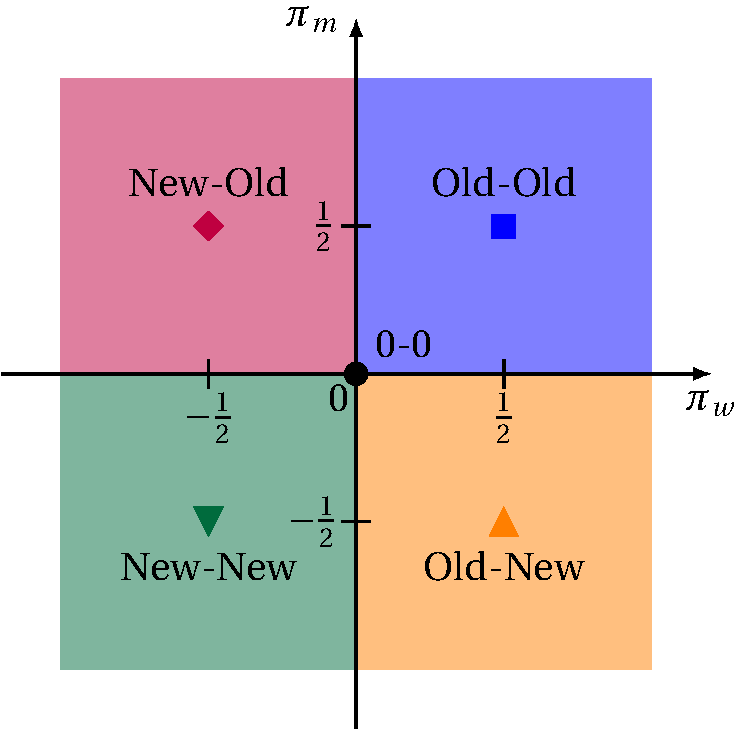
\includegraphics[width=0.5\textwidth]{fig1.pdf}
	\caption{\textbf{Parameter sets and legends for the different dispersal schemes.} \small The colors and markers are the same across all figures. The horizontal axis is the dispersal bias of the wild type, $\pi_w$ (positive values corresponding to preferential immigration into old-habitat patches), and the vertical axis that of the mutant, $\pi_m$. The markers are located at the parameter values used in the simulations.
		%: $\pi_m=\pi_w=0$ for unbiased dispersal (0-0; {\Large $\bullet$}), $\pi_m=\pi_w=0.5$ for a type-independent bias towards old-habitat patches (Old-Old; {\color{blue} $\blacksquare$}), $\pi_m=-0.5,\pi_w=0.5$ for a wild-type preference towards the old habitat, and a mutant-bias to the new habitat (Old-New; {\color{orange}$\blacktriangle$}), $\pi_m=\pi_w=-0.5$ for a type-independent bias towards the new habitat (New-New; {\color{darkgreen}$\blacktriangledown$}), and $\pi_m=0.5,\pi_w=-0.5$ for the mutant-bias towards the old habitat and a preference of the wild type for the new habitat (New-Old; {\color{purple}$\blacklozenge$}). 
		}
	\label{fig:disp_schemes}
\end{figure}

\linespread{1}
\begin{table}[t!]
	\begin{center}
		\begin{tabular}{c | P{6cm} | c | c}
			\textbf{Parameter} & \textbf{Interpretation} & \textbf{Range} & \textbf{Default value} \\
			\midrule
			$K_k$ & Carrying capacity in a patch of type $k$ & -- & \makecell{$K_{\text{old}}=1000$,\\ $K_{\text{new}}=500$} \\
			$\omega_j$ & \makecell{Expected per-capita number of\\ type $j$ offspring in the old habitat\\ before regulation} & $0\leq \omega^\text{old}_m < \omega^\text{old}_w$ & \makecell{$\omega^\text{old}_w = 1.5$,\\ $\omega^\text{old}_m=1.45$ {\footnotesize (weak sel.)},\\ $\omega^\text{old}_m=1.35$ {\footnotesize (strong sel.)}}\\
			$1+a_{\text{old}}$ & \makecell{Growth rate of the mutant\\ in the old habitat} & $-1\leq a_{\text{old}}$ & -- \\
			$1-r$ & \makecell{Mean number of wild-type offspring\\ in the new habitat} & $0<r\leq 1$ & \makecell{$0.75$\\ $(r=0.25)$}\\
			$1+a_{\text{new}}$ & \makecell{Growth rate of the mutant\\ in the new habitat} & $0<a_{\text{new}}$ & \makecell{$1.02$ \\ ($a_{\text{new}}=0.02$)} \\
			$m$ & Emigration probability & $0<m\leq 1$ & $0.06$\\
			$\pi_i$ & Type $i$ bias towards the old habitat & $\pi_i\in\mathbb{R}$ & see Fig.\ref{fig:disp_schemes}\\
			$\widehat{\pi}_i$ & Transformed dispersal bias of type $i$ & $0<\widehat{\pi}_i$ & see Fig.\ref{fig:disp_schemes}\\
			$M$ & Number of patches & $2\leq M$ & $10$\\
			$f_{\text{old}}$ & Frequency of old-habitat patches & $0\leq f_{\text{old}}\leq 1$ & $0.5$ \\
			$\theta$ & Mutation probability & $0 < \theta$ & $\frac{1}{25 M K_{\text{new}}}$\\
			$\tau$ & Time interval between two consecutive deterioration events& $0<\tau$ & $100$\\
			\midrule
			$\widehat{N}_{i}^{k}$ & \multicolumn{3}{p{11cm}}{Number of type $i$ individuals in type $k$ habitat patches at stationarity}  \\
			$\widetilde{N}_{i}^{k}$ & \multicolumn{3}{p{11cm}}{Number of type $i$ individuals in type $k$ habitat patches after dispersal}
		\end{tabular}
		\caption{\textbf{Model parameters.}}	
		\label{tab:parameters}
	\end{center}
\end{table}
\linespread{1.7}

\todo{to be moved} All the model parameters are summarized in Table~\ref{tab:parameters} along with the default parameter values and ranges. If not stated otherwise, the default parameter values are used for the stochastic simulations. 

\subsection*{Analysis steps}
We decompose our analysis into several steps of increasing complexity. 
\begin{enumerate}
	\item We first consider an environment that is constant over time, and heterogeneous over space, with a fraction $f_{\text{old}}$ of old-habitat patches and $1-f_{\text{old}}$ of new-habitat patches. The population is initiated with wild-type individuals at carrying capacity in old-habitat patches, and at the migration-selection equilibrium $\widehat{N}_w^{\text{new}}$ in new-habitat patches (see Section S1 in the SI for details), 
	and with a single mutant individual, either in an old- or in a new-habitat patch. There are no further mutations ($\theta = 0$), and we compute the \textit{probability of establishment} of a mutant lineage. 
	\item We then consider the same environmental setting, but initialize the population with only wild-type individuals. Mutants can appear by mutation during the simulation ($\theta >0$). We compute the \textit{probability of adaptation}, i.e. that, during a fixed time interval, a mutant appears by mutation and then establishes. 
	\item Finally, we consider the full scenario where each patch degrades one after the other, as described above. The environment is spatially and temporally variable. The population is initialized with only old-habitat patches, all at carrying capacity, with wild-type individuals only. We compute the \textit{probability of evolutionary rescue}, i.e. that a mutant appears by mutation and establishes before the population goes extinct. 
\end{enumerate}



%%%%%%%%%%%%%%%%%%%%%%%%%%
% Old habitat dynamics %%%
%%%%%%%%%%%%%%%%%%%%%%%%%%
\subsection*{Additional assumptions for the analytical part}
We make a few additional assumptions in the analytical part of our work; these assumptions are relaxed in the stochastic simulations. 

A key assumption to our mathematical analysis is that the mutant individuals are rare enough that their dynamics do not affect the wild-type population, at least during the establishment phase of the mutant lineage. The wild-type population sets a demographic context that affects mutants dynamics. The mathematical analysis therefore focuses on the population dynamics of the mutant population, considering the wild-type population as constant over time.\footnote{\florence{please check this is correct}}

We assume that the subpopulations in old-habitat patches are always at carrying capacity, i.e.\ that there are always enough offspring that are produced to at least replace all the parents. Denoting by $\widetilde{N}_{i}^{k}$ the number of type-$i$ individuals in a $k$-habitat patch right after dispersal, then the expected number of successful offspring of mutant individuals in this old-habitat patch (i.e., of offspring that survive density regulation and become adults in the next generation) is 
%
\begin{equation}\label{eq:sold}
K_{\text{old}}\, \frac{\omega^\text{old}_m \widetilde{N}^{\text{old}}_m}{\omega^\text{old}_w \widetilde{N}^{\text{old}}_w + \omega^\text{old}_m \widetilde{N}^{\text{old}}_m}
%
\approx K_{\text{old}}\, \frac{\omega^\text{old}_m \widetilde{N}^{\text{old}}_m}{\omega^\text{old}_w \widetilde{N}^{\text{old}}_w} 
%
\overset{\mathrm{def}}{=} \left(1 + a_{\text{old}}\right) \widetilde{N}^{\text{old}}_m \, .
\end{equation}
%
The approximation results from the assumption that mutants are rare compared to wild-type individuals in old-habitat patches. Eq.~\eqref{eq:sold} defines the per-capita expected growth rate of mutants in old-habitat patches, $a_{\text{old}}$. It depends on $\widetilde{N}^{\text{old}}_w$, the size of the local wild-type population right after dispersal, which is calculated in Section~\ref{sec:app:modeldyn} of the Supplementary Information (SI) (Eq.~\eqref{Seq:Ntildeold}).

\st{For the analysis, we also further assume that the number of successful offspring of mutant individuals is Poisson distributed, with mean $1+ a_{\text{old}}$. }\florence{com eback to this}

%\hl{The sign of this local growth rate depends on the value of $\widetilde{N}^{\text{old}}_w$, the size of the local wild-type population right after dispersal. Mutants are less fecund that wild-type individuals in old-habitat patches ($\omega^\text{old}_m < \omega^\text{old}_w$), yet the number of mutants can increase in old-habitat patches if $\widetilde{N}^{\text{old}}_w$ is low enough. In this case indeed, the population is far from carrying capacity, and the offspring of all types of individuals can make it to the next generation. Competition is fiercer as carrying capacity is nearer. }\footnote{\florence{I think this is more Results than Model}}. \linelabel{R1-14}The population dynamics of the wild type are analyzed explicitly in Section~\ref{sec:app:modeldyn} of the Supplementary Information (SI).

In new-habitat patches, on the contrary, we assume that population size remains much lower than carrying capacity, so that all offspring make it to the next generation (no regulation is necessary after reproduction).\footnote{\florence{I am getting rid of notation $r$}} The expected number of successful offspring of mutant individuals in a new-habitat patch, given that there are $\widetilde{N}^{\text{new}}_m$ mutants in the patch right after dispersal, is 
%
\begin{equation}\label{eq:defanew}
\omega_{m}^{\text{new}} \widetilde{N}^{\text{new}}_m = \left(1+a_{\text{new}} \right) \widetilde{N}^{\text{new}}_m,
\end{equation}
which defines $a_{\text{new}}$, the per-capita growth rate of mutants in new-habitat patches. This assumption constrains the differences in carrying capacities among old- and new-habitat patches under which our analysis remains valid. In particular, $K_{\text{new}}$ cannot be too much lower than $K_{\text{old}}$, because in this case, the flow of migrants from old- to new-habitat patches would substantially increase local population sizes in new-habitat patches. 

To summarize, for the analysis part, we assume that the number of successful offspring of mutant individuals are Poisson-distributed, with means $(1+ a_{\text{old}})$ in old-habitat patches, and $1+ a_{\text{new}}$ in new-habitat patches, where both quantities are treated as constant over time\footnote{\florence{please check this statement}}. \linelabel{R1-17}\linelabel{R2-13} These assumptions, made for the sake of mathematical analysis, are relaxed in our stochastic simulations.


\subsection*{Simulations}
The simulation algorithm implements the life cycle described above. We specify here the sampling distributions\footnote{\florence{please check the wording of this sentence}} that we use. 
\begin{enumerate}[label = (\roman*)]
	\item Dispersal: for each patch, a random number of dispersing individuals is drawn from a binomial distribution with success probability $m$.  %and sample size equal to the patch's current population size. [removed because obvious; and for consistency would have to be specified for all binomial dists] 
	The dispersing individuals from all patches are pooled together and redistributed into patches according to their type and the dispersal pattern. \linelabel{R2-18} For each type of individuals (wild-type and mutant), immigration patches are assigned by first drawing the number of individuals who immigrate into old-habitat patches from a binomial distribution with success probability $\frac{m_i^{\text{old}}}{m}$ (eq.~\eqref{eq:dispersal}), and then distributing these individuals uniformly at random over the old-habitat patches. The remaining dispersing individuals are then distributed uniformly a random into the new-habitat patches. 
	\item Reproduction: \linelabel{R2-19}In each patch, reproduction is simulated by drawing a Poisson distributed number for each type. The mean of this Poisson number is the product of the number of individuals of type $i$ in that patch times $\omega_i^k$, the mean number of offspring of a single individual of type $i$ in a patch of habitat $k$ (old or new). 
	All adults are then removed. 
	\item Mutation: the number of wild-type \linelabel{R2-20}offspring mutating into the mutant type is drawn from a binomial distribution, with success probability $\theta$, the mutation probability. 
	\item Density regulation: if the number of offspring in a patch is higher than the local carrying capacity ($K_k$ for a patch of habitat-type $k$ (old or new)), \linelabel{R1-25}patches, we sample $K_k$ individuals uniformly at random without replacement from the offspring population of the patch (hypergeometric sampling). Otherwise, the local population is left unchanged. 
\end{enumerate}	


% Initial conditions
%\paragraph{Initial conditions} 
%In Figs.~\ref{fig:vary_m_est}-\ref{fig:origin}, we simulate a heterogeneous environment that is constant in time, i.e. no patches deteriorate. Initial population sizes are $K_{\text{old}}$ wild-type individuals in old-habitat patches, and $\widehat{N}_w^{\text{new}}$ in new-habitat patches, which is the analytical stationary wild-type population size (see Section S1 in the SI for details). Simulations for Fig.~\ref{fig:vary_m_est} are started with initially one mutant either in a old- or a new-habitat patch and the corresponding wild-type population size is reduced by one; the mutation probability is set to zero. In \linelabel{R2-21} Figs.~\ref{fig:source_sink} and \ref{fig:origin}, mutants solely arise due to mutations. 

We consider that the mutant population has established if its total population size in patches of a given habitat type (old or new) is greater than $60\%$ the total carrying capacity of patches of that type ($(0.\chg{6} \times K_{\text{new}} \times M(1- f_{\text{old}}))$ for new-habitat patches, $(0.6\times K_{\text{old}}\times M f_{\text{old}})$  for old-habitat patches). \footnote{\florence{simulation duration in non-rescue scenarios?}}

Unless stated otherwise, the simulation results are averages of $10^5$ independent runs. All simulations are written in the C++ programming language and use the \textit{Gnu Scientific Library}. The codes and data to generate the figures are deposited on Gitlab\footnote{https://gitlab.com/pczuppon/evolutionary\_rescue\_and\_dispersal}.

%%%%%%%%%%%%%%%%%%%%%%%%%%%%%%%%%%%%%%%%%%%%%%%%%%%%%%%%%%%%%%%%%%%
%%%%%%%%%%%%%%%%% RESULTS %%%%%%%%%%%%%%%%%%%%%%%%%%%%%%%%%%%%%%%%%
%%%%%%%%%%%%%%%%%%%%%%%%%%%%%%%%%%%%%%%%%%%%%%%%%%%%%%%%%%%%%%%%%%%
\section*{Results}

% Removed because the different steps are now described above
%We investigate the effect of the different dispersal schemes on the probability of %successful adaptation and 
%evolutionary rescue. We first compute the \textit{establishment probability} of a single mutant individual arising either in an old- or in a new-habitat patch. \hl{We then link this probability to the dynamics of a source-sink system}\footnote{\florence{I don't understand what this means -- link?}}, i.e. a fixed environment with a certain number of old habitats (sources) and new-habitat patches (sinks). We derive an expression for the probability of a mutation to emerge and establish in a given time interval. We call this second quantity the \textit{probability of adaptation}. Lastly, we study the time-varying scenario where patches, one after \chg{another}, deteriorate. We consider a third quantity, the \textit{probability of evolutionary rescue}, which corresponds to the probability that a mutant appears by mutation and establishes in the new environment \chg{after} all patches have deteriorated. The theoretical results are complemented by stochastic simulations that support our predictions and help visualize the differences between the different dispersal schemes.

We proceed step-wise towards the computation of a probability of evolutionary rescue. For each step, we first present a mathematical analysis, for then compare our results to the output of simulations that relax the assumptions made for mathematical purposes. 


%%%%%%%%%%%%%%%%%%%%%%%%%%%%%%%
% Establishment Probability %%%
%%%%%%%%%%%%%%%%%%%%%%%%%%%%%%%
\subsection*{Establishment probability in a heterogeneous environment}\label{subsec:establishment}

In this first step, we consider that there is initially a single mutant individual in the population, located either in an old- or a new-habitat patch, and we compute the probability of establishment of the mutant population. In this step, we ignore further mutations and are only concerned with the fate of this single mutant lineage. 

\subsubsection*{Mathematical analysis}
The dynamics of the mutant population can be described by a two-type branching process. A key assumption of this framework is that \linelabel{R1-27}all mutants reproduce, disperse and die independently of each other. This is a reasonable assumption as long as the overall number of mutants is a lot smaller than the population size of the wild type. The two ``types'' in the name of method, two-type branching process, correspond to the two habitat types. The process tracks the \linelabel{R2-25}total number of mutants in old- and new-habitat patches at the end of each generation. As mentioned above, the numbers of successful offspring of mutant individuals, i.e., of offspring that survive density regulation and become adults at the next generation, are approximated by Poisson-distributed numbers, with means $(1+ a_{\text{old}})$ in old-habitat patches (eq.~\eqref{eq:sold} and eq.~\eqref{Seq:s_old}), and $1+ a_{\text{new}}$ in new-habitat patches (eq.~\eqref{eq:defanew}). After one generation, the mean number of successful offspring of a single mutant, either in an old- or a new-habitat patch, is then given by the following mean reproduction matrix:
%
\begin{equation}\label{eq:mean_repro}
	\bordermatrix{ ~ & \text{old patch} & \text{new patch} \cr
		\text{old patch} & \left(1-m_m^{\text{new}}\right) (1+a_{\text{old}}) & m_m^{\text{new}} (1+a_{\text{new}}) \cr
		\text{new patch} & m_m^{\text{old}} (1+a_{\text{old}}) & \left(1-m_m^{\text{old}}\right) (1+a_{\text{new}})
		}\ ,
\end{equation}
%
where the rows denote the parent locations, and the columns the patch type of the successful offspring. 
For example, the top-left entry is the probability for the parent to stay in an old-habitat patch ($1-m_m^{\text{new}}$, see eq.\eqref{eq:dispersal}) times the average number of successful offspring in these patches \linelabel{R2-26}(see Section~\ref{sec:app:modeldyn} in SI for the derivation of $a_{\text{old}}$ at the wild-type equilibrium). The other entries are obtained analogously.

\linelabel{R1-24}We denote by $\varphi_{\text{old}}$ (resp. $\varphi_{\text{new}}$) the probability of establishment of this two-type branching process when the mutant is initially located in a old- (resp. new-) habitat patch. This probability is computed by considering all possible ways of going extinct: the initial individual having $j$ successful offspring in a patch of type $k$, but all lineages descending from these $j$ offspring eventually go extinct; then summing over $k$ and $j$. The establishment probabilities $\varphi_{\text{old}}$ and $\varphi_{\text{new}}$ are then given by the unique positive solution of the following system of equations \citep[see][Chapters 5.3 and 5.6]{haccou_book}:
%
\begin{equation}\label{eq:ext_prob}
	\begin{aligned}
		1-\varphi_{\text{old}} &= \sum_{j=0}^{\infty}\left( \mathbf{P}(j \text{ successful offspring in old habitat})(1-\varphi_{\text{old}})^j \right. \\
		&\qquad \qquad \qquad \left.+ \mathbf{P}(j \text{successful offspring in new habitat})(1-\varphi_{\text{new}})^j\right)\\
		&=\exp\left[-\left(1-m^{\text{old}\to \text{new}}_m\right)(1+a_{\text{old}})\varphi_{\text{old}} - m^{\text{old}\to \text{new}}_m (1+a_{\text{new}}) \varphi_{\text{new}}\right]\, ,   \\
		1-\varphi_{\text{new}} &= \exp\left[-m^{\text{new}\to \text{old}}_m(1+a_{\text{old}})\varphi_{\text{old}} - \left(1-m^{\text{new}\to \text{old}}_m\right) (1+a_{\text{new}}) \varphi_{\text{new}}\right]\, .
	\end{aligned}
\end{equation}
This system of equations can be solved numerically. An analytical approximate solution is available in the case of weak selection and (potentially) weak dispersal (i.e. $a_{\text{old}},a_{\text{new}},m\ll 1$ needs to hold for at least two of the three parameters); see for example~\citet[Theorem~5.6]{haccou_book} for the general theory and \citet{tomasini_2018} for an application in a similar setting. The detailed derivation is presented in the SI, Section~\ref{sec:approxestabproba}. We find
\begin{equation}\label{eq:estab_approx}
	\begin{aligned}
		\varphi_{\text{old}} &\approx \qquad \quad \; \; \; \; a_{\text{old}}&+ & \quad a_{\text{old}} \frac{\left(1-f_{\text{old}}+\widehat{\pi}_m f_{\text{old}}\right)}{\sqrt{C}}(a_{\text{old}}-a_{\text{new}}) \\
		& & &  \; \; \; + \; \frac{m}{\sqrt{C}} \left(a_{\text{new}}(1-f_{\text{old}}) + a_{\text{old}}\widehat{\pi}_m f_{\text{old}} - (a_{\text{old}}-a_{\text{new}})(1-f_{\text{old}})\right) \, ,\\
		\varphi_{\text{new}} &\approx \underbrace{ a_{\text{new}}}_{\text{(1) local growth parameter}} &+ & \quad \underbrace{ a_{\text{new}} \frac{\left(1-f_{\text{old}}+\widehat{\pi}_m f_{\text{old}}\right)}{\sqrt{C}}(a_{\text{new}}-a_{\text{old}})}_{\text{(2) effect of the heterogeneous environment}} \\
	& & &  \underbrace{+\; \frac{m}{\sqrt{C}}\left( a_{\text{new}}(1-f_{\text{old}}) + a_{\text{old}} \widehat{\pi}_m f_{\text{old}} - (a_{\text{new}}-a_{\text{old}}) \widehat{\pi}_m f_{\text{old}} \right)\, ,}_{\text{(3) effect of dispersal: new patches $+$ old patches $-$ loss to the other patch type }}
	\end{aligned}
\end{equation}
where $C$ is a scaling constant that depends on $m,f_{\text{old}},\widehat{\pi}_m,a_{\text{old}}$ and $a_{\text{new}}$ through
\begin{equation}\label{eq:normalization}
	C = (1-f_{\text{old}}+\widehat{\pi}_m f_{\text{old}}) \left((1-f_{\text{old}})(a_{\text{new}}-a_{\text{old}}+m)^2 + \widehat{\pi}_m f_{\text{old}} (a_{\text{new}}-a_{\text{old}}-m)^2\right)\, . 
\end{equation}

The first term in the approximation of the establishment probabilities ($\varphi_{\text{old}}$ and $\varphi_{\text{new}}$) in eq.~\eqref{eq:estab_approx} describes the local growth depending on the habitat type under study. 
The second term captures the growth rate differences between the two habitat types.
The factor $(1-f_{\text{old}}+\widehat{\pi}_m f_{\text{old}})$ accounts for the biased dispersal patterns (when $\pi_m\neq 0$ so that $\widehat{\pi}_m\neq 1$). 
The third term in the equations corresponds to the direct effect of dispersal on the establishment probability. 
The first two summands in the bracket are the same for both establishment probabilities. They represent the general effect of dispersal due to the dynamics from new-habitat patches (first summand) and old-habitat patches (second summand). The dispersal bias induced by $\pi_m$ changes the relative impact of old- vs. new-habitat patches. 
Finally, the last summand in the bracket measures the growth rate loss (or gain) due to dispersal to the other patch type. It therefore differs between the two approximations.

Note that in these equations, the competition of the mutant with the wild type in old-habitat patches appears in the local growth rate $a_{\text{old}}$, defined in eq.~\eqref{eq:sold}. This quantity is not constant, but instead depends on the wild type population size in old-habitat patches, which itself depends on the wild type's dispersal and growth rate in both habitats \linelabel{R2-28}\chg{(see SI, Section S1)}.

If the emigration probability is zero ($m=0$), the subpopulations in each habitat evolve in isolation from each other and we recover Haldane's classical result for the establishment probability of a slightly advantageous mutant in new habitats: $\varphi_{\text{new}}=2a_{\text{new}}$ \citep{haldane_1927}. \linelabel{R1-69}\chg{In old-habitat patches, where the mutation is deleterious, we see that term (1) and (2) cancel each other so that the establishment probability is simply $\varphi_{\text{old}}=0$.} Furthermore,\francois{when the emigration probability is strictly positive (m>0)} in the case of \chg{unbiased} dispersal ($\pi_w=\pi_m=0$) and for equal number of old- and new-habitat patches ($f_{\text{old}}=1/2$), we obtain the approximation found in \cite{tomasini_2018} (compare system~\eqref{eq:estab_approx} to their eqs.~(4) and~(5)). Note that the approximation is independent of the actual number of patches, but only depends on the environmental configuration determined by the frequency of old-habitat patches $f_{\text{old}}$.

\subsubsection*{Comparison to simulations and qualitative behavior}
We compare in Fig.~\ref{fig:vary_m_est} our predictions from eqs.~\eqref{eq:ext_prob} and~\eqref{eq:estab_approx} to simulation results for different values of the emigration rate $m$. We find good agreement with the numerical solution of eq.~\eqref{eq:ext_prob} (solid lines). The approximation given in eq.~\eqref{eq:estab_approx} (dashed lines) deviates slightly from the simulation results in regions where $m,a_{\text{new}}$ and $a_{\text{old}}$ are not small, i.e. when the assumptions made in the analytical derivation do not hold anymore. 

\begin{figure}[t!]
	\centering
	\begin{subfigure}{.5\textwidth}
  		\centering
  		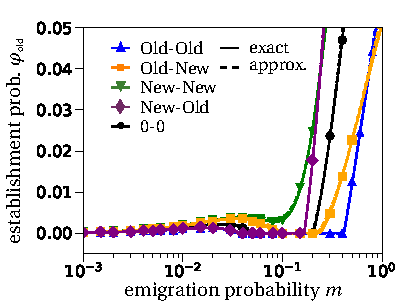
\includegraphics[width=\linewidth]{fig2a.pdf}
  		\caption{$\varphi_{\text{old}}$ with $\omega^\text{old}_m = 1.35$ (large fecundity difference)}
	\end{subfigure}%
	\begin{subfigure}{.5\textwidth}
 		 \centering
 		 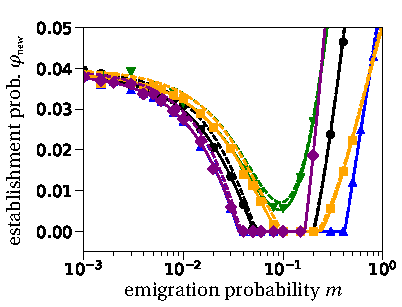
\includegraphics[width=\linewidth]{fig2b.pdf}
  		\caption{$\varphi_{\text{new}}$ with $\omega^\text{old}_m = 1.35$}
	\end{subfigure}
	\begin{subfigure}{.5\textwidth}
  		\centering
  		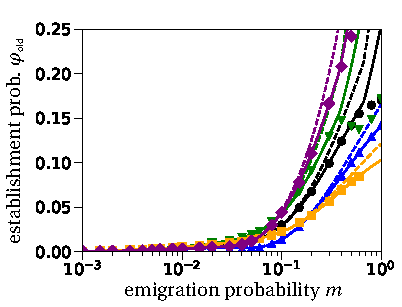
\includegraphics[width=\linewidth]{fig2c.pdf}
  		\caption{$\varphi_{\text{old}}$ with $\omega^\text{old}_m = 1.45$ (small fecundity difference)}
	\end{subfigure}%
	\begin{subfigure}{.5\textwidth}
 		 \centering
 		 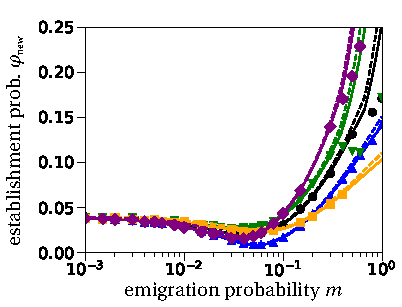
\includegraphics[width=\linewidth]{fig2d.pdf}
  		\caption{$\varphi_{\text{new}}$ with $\omega^\text{old}_m = 1.45$}
	\end{subfigure}
	\caption{\textbf{Establishment probability when varying the emigration rate.} \small We plot the theoretical results for $\varphi_{\text{old}}$ in (a) and (c), and for $\varphi_{\text{new}}$ in (b) and (d) for $\omega^\text{old}_m=1.35$ in (a), (b) and $\omega^\text{old}_m=1.45$ in (c), (d). Comparison with the results from stochastic simulations (symbols) show very good agreement with our approximation found in eq.~\eqref{eq:estab_approx} (dashed lines). The solid lines are the numerical solution of eq.~\eqref{eq:ext_prob}. The lines in (a) show a clear separation of the three regions of the establishment probability as discussed in the main text: {\color{change}(i) an initial increase due to higher probabilities of dispersal from old- to new-habitat patches; (ii) a local maximum due to increasing number of mutants emigrating from new-habitat patches; (iii) an increase due to relaxed competition in old-habitat patches, a result of wild-type emigration.}}
	\label{fig:vary_m_est}
\end{figure}

The qualitative dependence of the establishment probabilities $\varphi_{\text{old}}$ and $\varphi_{\text{new}}$ on the dispersal probability $m$ is similar for all dispersal schemes. The shape of the curve however strongly depends on the fecundity $\omega^\text{old}_m$ of mutants in the old habitat. Before discussing the differences between the dispersal schemes, we first provide a qualitative understanding of this general behavior.

For the probability of establishment of a single mutant in an old-habitat patch ($\varphi_{\text{old}}$), we observe up to three different regions, cf. Fig.~\ref{fig:vary_m_est}(a). This is in line with previous observations in the context of local adaptation \citep[e.g.][]{kawecki_1995,tomasini_2018} and evolutionary rescue \citep{uecker_2014}. We define the regions as follows: (i) an initial increase of the establishment probability at low dispersal rates $m$; (ii) a local maximum with a subsequent decrease of the establishment probability; (iii) an increase of the establishment probability for high dispersal rates.

A detailed assessment and explanation of the regions is provided in the SI, Section S2.1. Briefly, in region (i), the prevalent effect is the dispersal of mutants from old- to new-habitat patches where they are fitter than the wild type, thus increasing the establishment probability. This effect is mediated through the third term of the establishment probability in eq.~\eqref{eq:estab_approx}. 
Region (ii), beginning with the local maximum, is a result of two counteracting processes: %increased emigration of individuals from the old habitat and \linelabel{R2-30-1}\chg{an increasing probability of an individual that is born in a new habitat emigrates to an old-habitat patch.}
\linelabel{R2-30-1}\chg{If we increase the emigration probability $m$, a mutant is more likely to emigrate out of old-habitat patches and thus has a higher chance to establish. However, higher dispersal rates also have a negative effect on mutant establishment through \linelabel{R2-32}increasing the probability that a mutant migrates from a new- to an old-habitat patch. More precisely, the number of offspring in the new habitat on average is given by the product of the terms $(1-m_m^{\text{old}})$ and $(1+a_{\text{new}})$. This product can, for large emigration probabilities $m$, be smaller than $1$, i.e. a mutant in a new-habitat patch has on average less than one offspring. Finally, in region (iii), dispersal is so large that the population is close to being well-mixed. Most importantly, many wild-type individuals leave old-habitat patches which results in less competitive pressure in old-habitat patches. In this case the local growth rate of the mutant in these patches, $a_{\text{old}}$ (first term in eq.~\eqref{eq:estab_approx}), becomes positive. This effect called `relaxed competition'~\citep{uecker_2014}. The onset of this effect, in terms of the emigration probability $m$, is strongly dependent on the fecundity values of the mutant in the old habitat. The larger it is, the `earlier' (i.e. for smaller emigration rates $m$) relaxed competition becomes relevant.} 

%lowering competitive pressure in old-habitat patches \linelabel{R1-28-1}(see $\widetilde{N}_{\text{old}}^w$ from eqs.~(S7) and~(S8) in the SI). As a result, local growth rates of the mutant in old-habitat patches, \linelabel{R1-30} $a_{\text{old}}$, become larger. This effect was termed `relaxed competition' by \citet{uecker_2014}. 

%Depending on the onset of this effect, the establishment probability either has a local maximum or not, compare \ref{fig:vary_m_est}(a) and (c).
 
\chg{In line with this reasoning we find} that the width of region (ii) strongly depends on the fecundity of the mutant in the old habitat, $\omega^\text{old}_m$. If $\omega^\text{old}_m$ is high, the local growth rate of the mutant $a_{\text{old}}$ starts to increase at a lower dispersal rate 
%(see Fig.~S1). 
\chg{and }region (ii) disappears, as visible in Fig.~\ref{fig:vary_m_est}(c). In contrast, for low mutant fecundity values $\omega^\text{old}_m$, region (iii) might vanish (see Fig. S2 in SI). There, the mutant is strongly disadvantageous in old-habitat patches when compared to the wild type, and the wild-type population will always outcompete the mutant due to the much higher offspring numbers.

We analyze the qualitative behavior of the establishment probability of a mutant emerging in the new habitat, $\varphi_{\text{new}}$ in a similar way (Figs.~\ref{fig:vary_m_est}(b,d)). The establishment probability $\varphi_{\text{new}}$ decreases at low dispersal rates: Since we let the mutant start in a new-habitat patch, where it fares better than the wild type, there is no initial benefit due to dispersal (the third term in eq.~\eqref{eq:estab_approx} is negative for $\varphi_{\text{new}}$). The interpretation of region (ii), describing the trajectory for intermediate emigration rates $m$, is the same as for $\varphi_{\text{old}}$ above. For large emigration rates $m$, region (iii), the resulting establishment probability is a combination of the local growth rate and the dispersal effect, the first and third terms in eq.~\eqref{eq:estab_approx}. This is because the mutant can migrate to old-habitat patches, where it will enjoy relaxed competition. %%

\chg{Lastly, for large emigration probabilities $m$ in Fig.~\ref{fig:vary_m_est}(c,d) we observe a decrease in the establishment probability of the simulation results of the New-New dispersal scheme (and to a lesser extent in the unbiased scheme). This is explained by `gene swamping' whereby a to large number of immigrants of a less-well adapted type (wild type) inhibits the establishment of a locally better adapted type (mutant) \citep{nagylaki_1978,lenormand_2002}. Here, gene swamping occurs because of the different carrying capacities of the two patch types, $K_{\text{new}}<K_{\text{old}}$. A proper analysis of the gene swamping regime, where density-dependence in new-habitat patches is important, is beyond the scope of this manuscript, but see for instance \citet{tomasini_2018} and Section S5 in the SI where such a situation is studied.}\footnote{\pete{If I do not mention gene swamping here, I think people will wonder what this effect is and misinterpret it as a late relaxed competition effect.}}

\subsubsection*{Comparison of dispersal schemes}

We now compare the establishment probabilities for the different dispersal schemes. 
We consistently observe that \chg{a bias towards the new habitat (New-New} in Fig.~\ref{fig:vary_m_est}) enhances establishment when compared to the \chg{unbiased} dispersal scheme (0-0). This can be attributed to two reasons: (1) the mutant is more likely to disperse to the new habitat where it outcompetes the wild type (stronger weighting of new-habitat patches in the third term in eq.~\eqref{eq:estab_approx}); and (2) since the wild type prefers to settle in new-habitat patches ($\pi_w<0$), individuals in old-habitat patches experience relaxed competition for lower dispersal rates $m$, thus increasing the local growth rate $a_{\text{old}}$, i.e. region (iii) is shifted to the left. An analogous (but reversed) argument explains why \chg{a bias towards the old habitat (Old-Old}) is always lower than the \chg{unbiased} dispersal scheme. 

The effect of \chg{the asymmetric dispersal scheme Old-New}, where each type has a bias to move to the habitat where it is relatively fitter than the other type, is more involved. We disentangle the effects separately for each region. In region (i) at low emigration probabilities, the curve is almost identical to that of the \chg{New-New} pattern. The mutant preference \chg{(new habitats)} of these two dispersal modes is the same. The movement of the rare mutant is the prevailing process in this parameter regime, which explains the alignment of the \chg{corresponding} curves. 
For intermediate dispersal rates, region (ii), the effect of the heterogeneous environment (second term in eq.~\eqref{eq:estab_approx}) becomes stronger, i.e. the local growth rate $a_{\text{old}}$ increases because of relaxed competition in old-habitat patches. 
For the \chg{Old-New scheme}, the\linelabel{R2-30-3} wild type is more likely to immigrate into old-habitat patches and to increase the population size in these locations \linelabel{R1-31}\chg{when compared to the New-New dispersal scheme}. This reduces the effect of relaxed competition. Therefore, the \chg{Old-New line} drops below the \chg{New-New} curve and even starts to decrease (Fig.~\ref{fig:vary_m_est}(a)). For high emigration probabilities $m$, region (iii), the competitive pressure in old-habitat patches relaxes. Again, this region is dominated by the movement of wild-type individuals. In the \chg{unbiased} dispersal scheme, the wild type has a lower likelihood to be in old-habitat patches than with the \chg{Old-New} scheme, explaining the \chg{order of these} curves. 
For very large dispersal rates, also\francois{moreover?} the \chg{Old-Old} scheme can lead to higher values of $\varphi_{\text{old}}$ than \chg{the type-dependent preference Old-New}, cf. Fig.~\ref{fig:vary_m_est}(c). For these parameters, the mutant has a larger growth rate in old- than in the new-habitat patches ($a_{\text{old}}>a_{\text{new}}$). It is therefore beneficial for the mutant to \linelabel{R2-30-4}\chg{be in} old-habitat patches. 

Finally, for the \chg{asymmetric dispersal scheme New-Old, where the types have a bias to the habitat they are less well adapted to, }we see that for low dispersal rates $m$ the results match those obtained under the \chg{Old-Old} scheme. The mutant preferences being the same, this again shows that this region is dominated by the mutant's dispersal behavior. For intermediate to large dispersal rates though, the \chg{New-Old} scheme results in the largest establishment probabilities. This is explained by the effect of strongly relaxed competition (wild-type individuals preferentially move into the new habitat) and the bias of mutants to disperse into old-habitat patches where their number of offspring individuals is now very large. %Overall, this results in the highest establishment probabilities of all dispersal schemes. %We note though that the term `maladaptive dispersal' might be misleading for large dispersal values, since here the growth rate of the mutant in old-habitat patches, $a_{\text{old}}$, is actually larger than the growth rate in new-habitat patches, $a_{\text{new}}$. 

%%%%%%%%%%%%%%%%%%%%%%%%%%%%%%%
% Emergence probability %%%%%%%
%%%%%%%%%%%%%%%%%%%%%%%%%%%%%%%
\subsection*{Probability of adaptation in a heterogeneous environment} \label{subsec:source_sink}

We now study the probability of adaptation when mutations occur recurrently. As in the previous section, we consider a heterogeneous environment with a fixed number of old- and new-habitat patches. This is effectively a source-sink system \citep{holt_1985,pulliam_1988}, where old- and new-habitat patches correspond to sources and sinks for the wild type, respectively. In the previous section, we initialized the system with one mutant in either an old- or a new-habitat patch and computed the establishment probability. Now, we let mutants appear randomly within a certain time frame. The last time point at which a mutation can occur is denoted by $t_{\text{fin}}$.
Later, in the analysis of the probability for evolutionary rescue, this time will be replaced by the time between two consecutive patch deterioration events, $\tau$.\footnote{\pete{I think we can get rid of this last sentence. Thoughts?}\francois{Yes.}}

The probability of adaptation in this setting, $P_{\mathrm{adapt}}$, is given by
\begin{equation}\label{eq:source_sink}
	P_{\mathrm{adapt}} = 1 - \exp\left(-\theta t_{\text{fin}} M \left(\underbrace{\varphi_{\text{old}} f_{\text{old}} K_{\text{old}}}_{\text{old habitat contribution}} + \underbrace{\varphi_{\text{new}} (1-f_{\text{old}}) \widehat{N}_w^{\text{new}}}_{\text{new habitat contribution}}\right)\right)\, .	
\end{equation}
In words, the right-hand side is one minus the probability of no mutant establishing within the $[0, t_{\text{fin}}]$ time interval.
More precisely, the exponential is the probability of zero successes of a Poisson distribution. The rate of this Poisson distribution is given by the expected number of successfully emerging mutant lineages until time $t_{\text{fin}}$. \linelabel{R2-34}\chg{Assuming a Poisson distribution for the number of successful mutant lineages is an approximation of a Binomial distribution with large sample size (the wild-type populations $t_{\text{fin}} M f_{\text{old}} K_{\text{old}}$ in the old and approximately $t_{\text{fin}} M (1-f_{\text{old}}) \widehat{N}_w^{\text{new}}$ in the new habitats, see SI eq.~(S5)) with small success probability (the establishment probabilities $\varphi_{k}$). The sample size denotes the number of mutations in the system until time $t_{\text{fin}}$ and each of these mutants has, independently of each other (another approximation), has a survival probability of $\varphi_{k}$, dependent on the habitat it is born in.}
%Correctly, at least in the old habitat, one would have a Binomial distribution with success probability $\theta \varphi_{\text{old}}$ and sample size $t_{\text{fin}}M f_{\text{old}} K_{\text{old}}$ which is well approximated by a Poisson distribution for large sample sizes and small success probabilities. Due to the varying population size in the new habitat, the exact probability for successful lineages emerging from that habitat type is more difficult to compute. Yet again, on average this number is well approximated by the a Poisson distribution with a rate as stated above.}\footnote{\pete{This is the long explanation. I would shorten but if you think it is worth keeping a long explanation (as suggested by the reviewer) we can leave it as it is.}}
Note also, that for $t_{\text{fin}}$ tending to infinity, there will almost surely be a successful mutant so that $P_{\text{adapt}}=1$. \\
%For finite values of $t_{\text{fin}}$, the average number of mutations that appear until that time is given by the product of the mutation probability $\theta$, the length of the time window of interest $t_{\text{fin}}$, the number of patches $M$ and the stationary number of wild-type individuals present in the different habitats, that is $K$ and $\widehat{N}_w^{\text{new}}$ for old- and new-habitat patches, respectively (cf. SI eq.~(S5)). Once such a mutant appears, it then has the previously computed establishment probability $\varphi_{k}$ to establish, depending on the patch type $k$ (old or new) it arises in. This explains the factor $\varphi_k$ in the exponential.  \\

In Fig.~\ref{fig:source_sink} we compare our predictions to simulation results. The shape of the probability of adaptation as function of the emigration probability $m$ depends on the fecundity of the mutant in old-habitat patches, $\omega^\text{old}_m$ (Figs.~\ref{fig:source_sink}(a,c)). This is similar to the behavior of the establishment probability $\varphi_{\text{old}}$ in Fig.~\ref{fig:vary_m_est}. Likewise, the qualitative effects of the different dispersal schemes are comparable to the ones observed for the establishment probability. \linelabel{R1-33}\chg{This holds because the probability of adaptation, $P_{\text{adapt}}$, is given by $1-\exp(-C_1 \varphi_{\text{old}} -C_2 \varphi_{\text{new}})$ where two constants $C_1$ and $C_2$ depend on the dispersal scheme (see eq.~\eqref{eq:source_sink}). \linelabel{R2-35}The small differences in the ranking of the dispersal schemes between subfigures Figs.~\ref{fig:vary_m_est}(c) and Figs.~\ref{fig:source_sink}(c) can be explained by the mutational input, i.e. larger stationary populations sizes of the wild type in new habitats, $\widehat{N}_w^{\text{new}}$ result in more mutations during the observed time frame. This population size is altered by the different dispersal schemes, most importantly it is largest for the wild type having a bias towards old habitats, i.e. the Old-Old and the Old-New dispersal schemes.} 

\begin{figure}[t!]
	\centering
		\begin{subfigure}{.5\textwidth}
 		 \centering
 		 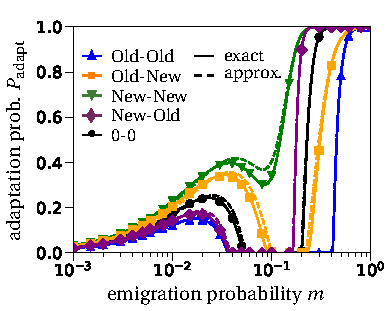
\includegraphics[width=\linewidth]{fig3a.pdf}
  		\caption{$\omega^\text{old}_m=1.35$ (large fecundity difference)}
	\end{subfigure}%
	    \begin{subfigure}{.5\textwidth}
 		 \centering
 		 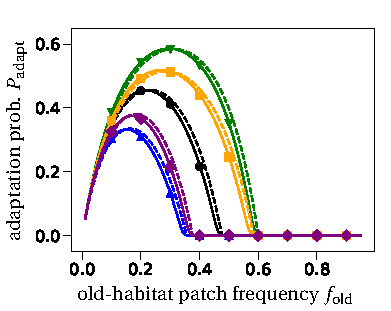
\includegraphics[width=\linewidth]{fig3b.pdf}
  		\caption{$\omega^\text{old}_m=1.35$}
	\end{subfigure}
	\begin{subfigure}{.5\textwidth}
 		 \centering
 		 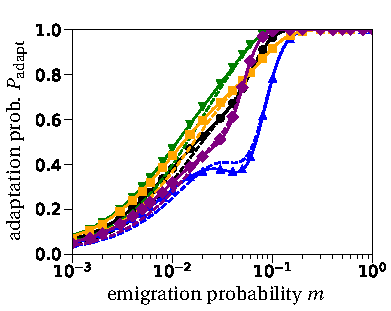
\includegraphics[width=\linewidth]{fig3c.pdf}
  		\caption{$\omega^\text{old}_m=1.45$  (small fecundity difference)}
	\end{subfigure}%
	\begin{subfigure}{.5\textwidth}
  		\centering
  		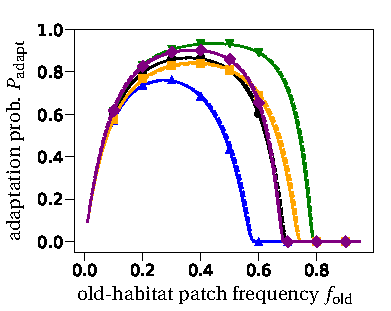
\includegraphics[width=\linewidth]{fig3d.pdf}
  		\caption{$\omega^\text{old}_m=1.45$}
	\end{subfigure}
	\caption{\textbf{Probability of adaptation in a heterogeneous environment.} \small In (a) and (c), we vary the emigration rate $m$ and observe a similar qualitative behavior as for the establishment probability $\varphi_k$ in Fig.~\ref{fig:vary_m_est}. In (b) and (d), we vary the frequency of old-habitat patches. The maximum is the result of two counteracting processes. The higher the number of old-habitat patches (the greater $f_{\text{old}}$), the larger the wild-type population. As a consequence, more mutants appear in the studied time-frame. In contrast, the less old-patch habitats there are in the environment (the lower $f_{\text{old}}$), the higher the probability of successful establishment of a mutant population. The curves labeled `approx.' are given by eq.~\eqref{eq:source_sink}, the exact solution refers to solving the establishment probabilities $\varphi_k$ from eq.~\eqref{eq:ext_prob} numerically and plugging these solutions into eq.~\eqref{eq:source_sink}. In all panels, the mutation probability is $u=1/(M K)$ and the final time for a mutant to appear is $t_{\text{fin}}=100$. }
	\label{fig:source_sink}
\end{figure}

In subfigures (b) and (d), we plot the probability of adaptation as a function of the frequency of old-habitat patches $f_{\text{old}}$. We observe a maximum which is the result of two effects: (1) the likelihood for a mutation to appear increases with the number of wild-type individuals present in the system, which is highest for high frequencies of old-habitat patches $f_{\text{old}}$, and (2) the probability of establishment of a mutant decreases with the number of old-habitat patches. 

The different dispersal schemes alter both effects. \chg{A general bias towards the new habitat (New-New)}, when compared to \chg{unbiased} dispersal (0-0), always shifts the maximum to higher frequencies of old habitats while also increasing its quantitative value. \chg{Since for the New-New dispersal scheme, both types prefer settling in new-habitat patches ($\pi_w,\pi_m<0$), the local population before reproduction in these patches is increased. Thus, the overall population size is higher compared to the other dispersal schemes and therefore a higher number of mutants is generated under this scheme.} Additionally, the probability of establishment is also increased for \chg{the New-New} dispersal scheme, further increasing the probability of adaptation (see also the discussion around Fig.~\ref{fig:vary_m_est}). Again, a reversed argument explains why \chg{the general preference for old-habitat patches (Old-Old)} always yields lower probabilities of adaptation than \chg{unbiased} dispersal.  


%%%%%%%%%%%%%%%%%%%%%%%%%%%%%%%
% Origin of rescue mutation %%%
%%%%%%%%%%%%%%%%%%%%%%%%%%%%%%%
\subsection*{Habitat of origin of the adaptive mutation}
We now identify the habitat type where the successful mutation arises. The established mutant population often arises from a single mutant that is born in an old- or in a new-habitat patch. However, the rescued population can sometimes be traced back to two (or more) mutant individuals, \chg{at least} one from either patch type. \linelabel{R1-35}\chg{This is a special type of a soft selective sweep \citep[see][for a review]{hermisson_2017}. The approximate probability to observe a soft sweep from mutants from both habitat types is 
\begin{equation}\label{eq:origin}
    \begin{aligned}
	&\mathbf{P}\big(\text{successful adaptation from old habitat}\big)\ \mathbf{P}\big(\text{successful adaptation from new habitat}\big) \\
	& \qquad \qquad \approx \left(1 - \exp\left(-\theta t_{\text{fin}} M \varphi_{\text{old}} f_{\text{old}} K\right)\right)\left(1- \exp\left(-\theta t_{\text{fin}} M \varphi_{\text{new}} (1-f_{\text{old}}) \widehat{N}_w^{\text{new}}\right)\right)\, .
	\end{aligned}
\end{equation} 
}
\linelabel{R1-36}\chg{The approximation uses our basic assumption that different mutant individuals and consequently also the offspring of different mutants do not affect each others dynamics (branching process). In the simulations, we label a run as a soft sweep from mutants arising in different locations if these lineages are still alive after $1000$ generations. This ensures that we do not count any false-positives where a mutant in one of the habitats has just arisen right before the mutant population exceeds the establishment threshold.}

%The probabilities for the other two scenarios can be computed analogously. 
In Fig.~\ref{fig:origin} we compare simulation results with our predictions for the origin of a successful mutant when varying the old habitat frequency $f_{\text{old}}$. \chg{\linelabel{R2-36}We see that for both mutant fecundity values most successful mutations arise in old-habitat patches. The difference in the input from the two different patches is the factor $\varphi_{k} \widehat{N}_w^k f_k$. In Fig.~SX we plot the establishment probability $\varphi_k$ and the stationary population sizes $\widehat{N}_w^k$ when varying the frequency of old-habitat patches $f_{\text{old}}$. We see that the establishment probability for mutants arising in new-habitat patches, $\varphi_{\text{new}}$, is always larger than the corresponding probability for mutants from old-habitat patches, $\varphi_{\text{old}}$. Conversely, the stationary population size of the wild type in the old habitat measured over the whole environment is always larger then that of the wild type in new habitats. Combining these two observations we find that for this choice of parameters the mutational input, i.e. the absolute number of rescue mutants, has a larger influence on the origin of the rescue mutant than the corresponding establishment probability.}

%Even for a relatively strong fecundity disadvantage of the mutant in the old habitat, i.e. $\omega^\text{old}_m$ is $10\%$ smaller than $\omega^\text{old}_w$, we find that most successful mutations arise in old-habitat patches (Fig.~\ref{fig:origin}(a)). Decreasing the fecundity disadvantage of the mutant by increasing its fecundity $\omega^\text{old}_m$ further increases the number of successful mutant lineages from old-habitat patches (Fig.~\ref{fig:origin}(b)). 
%If we instead increase the fecundity difference in old habitats by decreasing $\omega^\text{old}_m$, we observe the opposite, i.e. \chg{the two lines approach each other} (see Fig.~S4 in SI).

\begin{figure}[t!]
	\centering
	\begin{subfigure}{.5\textwidth}
 		 \centering
 		 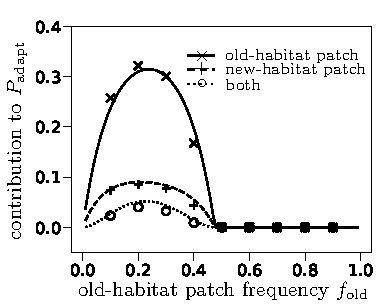
\includegraphics[width=\linewidth]{fig4a.pdf}
  		\caption{$w_m = 1.35$ (large fecundity difference)}
	\end{subfigure}%
	\begin{subfigure}{.5\textwidth}
  		\centering
  		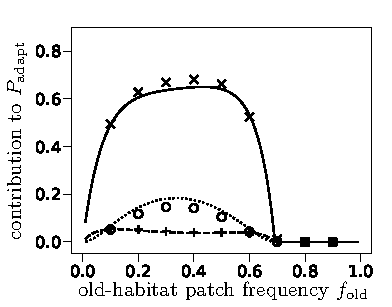
\includegraphics[width=\linewidth]{fig4b.pdf}
  		\caption{$w_m = 1.45$ (small fecundity difference)}
	\end{subfigure}
	\caption{\textbf{Origin of the adaptive mutant.} \small The origin of the adaptive mutant is strongly affected by the fecundity differences in the old habitat. If the difference is large as illustrated in panel (a), mutants appear more often in old-habitat patches than in new-habitat patches. Still, mutants arising in new-habitat patches contribute to the overall probability of adaptation. If fecundity differences are small like in panel (b), the successful mutant largely arises in old-habitat patches. In this case, the contribution from new-habitat patches is negligible. Circles correspond to simulations identified as soft selective sweeps with (at least) one lineage \francois{successful mutation} arising in an old- and one in a new-habitat patch. The curves are given by eq.~\eqref{eq:origin} (or the adjusted versions of it) under the unbiased dispersal scheme ($\pi_w=\pi_m=0$). Note the different scaling on the y-axes.}
	\label{fig:origin}
\end{figure}

%%%%%%%%%%%%%%%%%%%%%%%%%%%%%%%
% Evolutionary Rescue %%%%%%%%%
%%%%%%%%%%%%%%%%%%%%%%%%%%%%%%%
\subsection*{Evolutionary rescue}
Finally, we consider a time-inhomogeneous environment where patches deteriorate one after \chg{another} at regular time intervals $\tau$, until all patches have switched to the new habitat. If the wild-type population fails to generate a successful mutant, the population will \chg{inevitably} go extinct. The probability of evolutionary rescue is therefore tightly linked to the probabilities of adaptation and establishment that we have computed in eqs.~\eqref{eq:estab_approx} and~\eqref{eq:source_sink}. Typically, in formulas expressing the probability of evolutionary rescue, one splits the contributions into mutations arising \textit{de novo} and evolutionary rescue due to standing genetic variation, i.e. mutations that are present in the population before the environmental change \citep{alexander_2014}. We will discuss the effect of standing genetic variation in our system in the following section. For now, we focus on evolutionary rescue due to de novo mutations. We approximate the probability of evolutionary rescue, denoted by $P_{\text{rescue}}$, as
\begin{equation}\label{eq:evol_rescue}
    \begin{aligned}
		P_{\text{rescue}} &\approx 1-\exp\left(- \theta \sum_{i=0}^{M-2} \left(\underbrace{\varphi_{\text{old}}\left(f_{\text{old}}(i)\right) \sum_{j=i\tau}^{(i+1)\tau -1} N_w^{\text{old}}(j)}_{\text{old habitat contribution}} + \underbrace{\varphi_{\text{new}}(f_{\text{old}}(i)) \sum_{j=i\tau}^{(i+1)\tau -1} N_w^{\text{new}}(j)}_{\text{new habitat contribution}}\right)\right.\\
		&\qquad\qquad \qquad\qquad\qquad\qquad\qquad \qquad \qquad \qquad\quad  \left.\underbrace{-\theta \varphi_{\text{new}}(0) \sum_{j = \tau (M-1) }^\infty  N_w^{\text{new}}(j)}_{\text{contribution after the last patch deteriorated}}\right),
	\end{aligned}
\end{equation}
where \linelabel{R1-40}$f_{\text{old}}(i) = (M-i-1)/M$ is the frequency of old-habitat patches after the $(i+1)-$th deterioration event\linelabel{R1-39}\chg{, the establishment probability is given as a function of the patch frequency, $\varphi_k(f_{\text{old}}(i))$,} and $N_w^{k}(j)$ denotes the overall number of wild-type individuals living in habitat $k$ (old or new) in generation~$j$ \chg{(see SI, Section S1 for an approximation)}. The interpretation of this equation is the same as for eq.~\eqref{eq:source_sink}. The only difference is that we now need to account for a changing environment, which alters the population sizes, $N_w^k$, and the establishment probabilities $\varphi_k$ \chg{over time}. In the formula, these changes are accounted for by the sums that iterate through the (discrete) time steps and by the time dependence of the corresponding quantities. We further note that we follow the \chg{expected value of} the wild-type population size deterministically over time, instead of assuming it to be already in its steady state as in eq.~\eqref{eq:source_sink} \chg{(see also Section \ref{sec:app:modeldyn} in the SI)}.

As visible in Fig.~\ref{fig:rescue}, the approximation explains the \linelabel{R1-42}\chg{order of dispersal schemes}. Yet, it does not accurately predict the simulated data. This discrepancy can be explained: in the formula we \linelabel{R2-42}\chg{assume that for a mutant born in a certain patch configuration, say with $j$ old-habitat patches, the environment does not change anymore. That is, a mutant born in patch-type $k$ (old or new) in this environment contributes $\varphi_{k}(j)$ to the probability of evolutionary rescue despite further patches deteriorating. Thus, this mutants probability of establishment is underestimated. This is especially true for mutants that emerge just before a deterioration event. These mutants are more likely to establish during the subsequent environmental configuration giving them a higher probability of survival than approximated by our formula. Additionally, $\varphi_k(j)$ assumes stationary wild-type population sizes and therefore does not reflect the decreasing wild-type population size right after the deterioration of a patch.} 
%However, mutants that arise very shortly before a deterioration event just need to survive until this event happens and are thus carried over to the following environmental configuration with a higher probability than predicted by our formula. 
This explains why the simulation results are higher than our approximation. 
%which ignores these ``left-over'' mutants present prior to the deterioration event. 
\chg{A time-dependent establishment probability could account for these effects but unfortunately is not amenable to approximations in our framework.}
%As a result, instead of assuming a constant establishment probability between two deterioration events, we should rather use a time-dependent establishment probability -- which can however not be approximated in our general framework. 
\linelabel{R1-43}\chg{In \citet{uecker_2014}, scenarios with an accessible time-dependent solution were studied, more precisely situations with either full mixing of the global population ($m=1$) or a non-viable mutant in old-habitat patches ($\omega^\text{old}_m=0$).}

\begin{figure}[t!]
	\centering
	\begin{subfigure}{.5\textwidth}
  		\centering
  		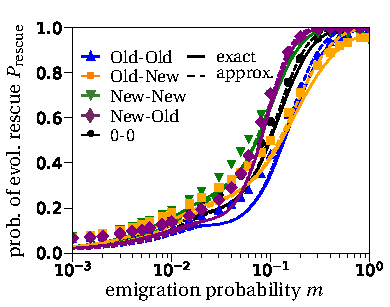
\includegraphics[width=\linewidth]{fig5a.pdf}
  		\caption{$\omega^\text{old}_m=1.45$ (small fecundity difference)}
	\end{subfigure}%
	\begin{subfigure}{.5\textwidth}
  		\centering
  		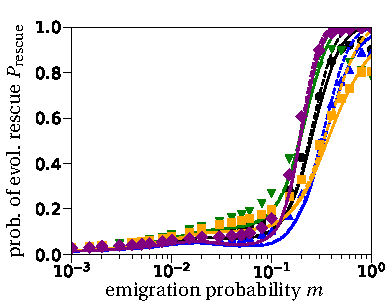
\includegraphics[width=\linewidth]{fig5b.pdf}
  		\caption{$\omega^\text{old}_m=1.35$ (large fecundity difference)}
	\end{subfigure}
	\begin{subfigure}{.5\textwidth}
  		\centering
  		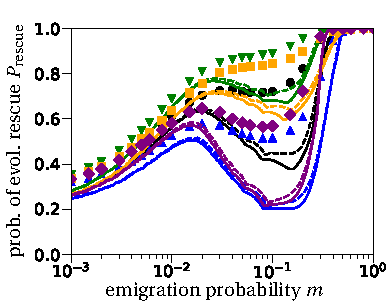
\includegraphics[width=\linewidth]{fig5c.pdf}
  		\caption{$\omega^\text{old}_m=1.1$ (very large fecundity difference)}
	\end{subfigure}%
	\begin{subfigure}{.5\textwidth}
  		\centering
  		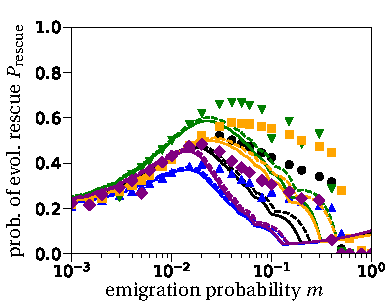
\includegraphics[width=\linewidth]{fig5d.pdf}
  		\caption{$\omega^\text{old}_m=0$ (lethal mutant)}
	\end{subfigure}
	\caption{\textbf{The probability of evolutionary rescue compared to simulation results.} \small Our predictions, computed with eq.~\eqref{eq:evol_rescue}, match the qualitative behavior of the simulated data for the probability of evolutionary rescue. All rankings of the dispersal schemes align well. Quantitatively though, we find that our predictions tend to underestimate the simulated data. In (a,b) the mutation probability is set to $u=1/(25MK_{\text{new}})$ while in (c,d) it is $u=1/(MK_{\text{new}})$. The label `exact' refers to the exact solution of eq.~\eqref{eq:ext_prob} which is then plugged into the approximation of the probability of evolutionary rescue in eq.~\eqref{eq:evol_rescue}.}
	\label{fig:rescue}
\end{figure}

The different dispersal schemes exhibit substantial differences. The dispersal schemes affect the dispersal pattern of both types and as such alter their respective population dynamics. Both small and large fecundity differences in the old habitat, $\omega^\text{old}_m=1.45$ and $\omega^\text{old}_m=1.35$, conserve the ranking of dispersal schemes obtained for the probabilities of establishment and adaptation\footnote{\francois{difficult to follow}\pete{We could also get rid of the explict description of the figure and remove the following sentence}}: \linelabel{R2-43}\chg{New-New (green) is higher than unbiased dispersal (black) which is higher than Old-Old (blue), with Old-New decreasing and New-Old increasing their positions with increasing emigration probability $m$}, cf. Fig.~\ref{fig:rescue}(a,b). Based on our discussion of the same behavior in Fig.~\ref{fig:vary_m_est}(a,c), \linelabel{R2-44}\chg{i.e. the change in hierarchy of the dispersal schemes Old-New and New-Old,} The most influential factor in these parameter sets is the growth rate of the mutant in old-habitat patches, $a_{\text{old}}$, \chg{as discussed around Fig.~\ref{fig:vary_m_est}.} \chg{The ranking of the symmetric dispersal schemes is mostly determined by the mutant dispersal bias.}

For very large fecundity differences in the old habitat ($\omega^\text{old}_m = 1.1$ and $\omega^\text{old}_m=0$), the ranking of dispersal schemes is the same for all emigration probabilities; from highest to lowest, we find \chg{New-New, Old-New, unbiased dispersal, New-Old, and Old-Old} (cf. Fig.~\ref{fig:rescue}(c,d)). In this parameter setting, the probability of evolutionary rescue is dominated by the dispersal behavior of the mutant. Since the mutant is barely viable in old-habitat patches, it is always preferential for it to disperse towards new-habitat patches. Two schemes follow this rule, \chg{the New-New and Old-New dispersal scheme}, but differ in the preference of the wild type. 
Since wild-type individuals also preferentially disperse to new-habitat patches under \chg{the New-New scheme}, more individuals are present in those patches. Therefore, the total amount of mutations over the deterioration time is increased which generates more mutants on average. This explains the New-New dispersal scheme being consistently higher than the Old-New dispersal scheme.
%This effect is even stronger for large dispersal rates that increase the wild-type population size in the whole environment. Together with the effect of relaxed competition, this explains the strong increase of the \chg{New-Old}, and the \chg{unbiased} dispersal scheme for large emigration probabilities $m$ in Fig.~\ref{fig:rescue}(c). 

Lastly, the probability of evolutionary rescue often reaches a local (or global) maximum for intermediate emigration probabilities (Figs.~\ref{fig:rescue}(c,d)). This extends previous results \citep{uecker_2014,tomasini_2019} to arbitrary dispersal schemes affecting the immigration process. The maximum can be attributed to the interaction of the three regions we identified when analyzing the establishment probability $\varphi_k$ (see also Fig.~\ref{fig:vary_m_est}). As such it is a result of the largely positive effect of dispersal (initial increase of the probability of evolutionary rescue) and the negative effect of population mixing \chg{(dispersal to old patches)}. \footnote{\francois{This discussion is still difficult.}}

\subsection*{Habitat of origin of the rescue mutant and standing genetic variation}
Similar to what \chg{we} found for the probability of adaptation, rescue mutants mainly originate from old-habitat patches. Mutations are more likely to appear in the more populated patches (old-habitat). However, a low mutant fecundity $\omega^\text{old}_m$ decreases the chance of establishment of these mutants that appear in old-habitat patches (compare black and yellow symbols in Fig.~\ref{fig:sgv}(a)). Lower fecundity values $\omega^\text{old}_m$ therefore comparatively increase the probability for the rescue mutation to have appeared in the already deteriorated habitat, i.e. in new-habitat patches. \linelabel{R1-35-2}\chg{The probability of a soft selective sweep for evolutionary rescue from mutants of the different habitat types is very low (circles in Fig.~\ref{fig:sgv}(a)). Our choice of a small mutation rate implies a hard selective sweep regime ($\theta K_{\text{old}} M = 0.08<1$) \citep{wilson_2018,hermisson_2017}. }

\begin{figure}[t]
	\centering
		\begin{subfigure}{.5\textwidth}
 		 \centering
 		 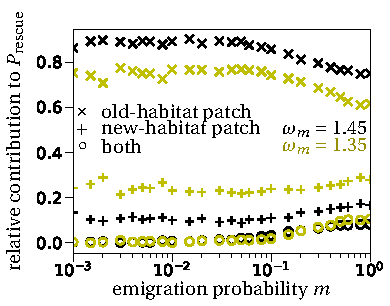
\includegraphics[width=\linewidth]{fig6a.pdf}
  		\caption{}
	\end{subfigure}%
    \begin{subfigure}{.5\textwidth}
 		 \centering
 		 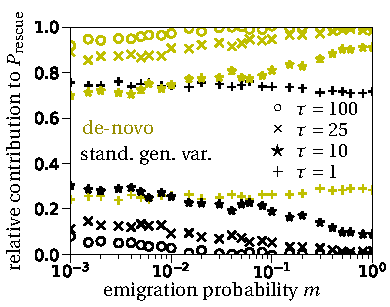
\includegraphics[width=\linewidth]{fig6b.pdf}
  		\caption{}
	\end{subfigure}
	\caption{\textbf{Habitat of origin of the rescue mutation and the impact of standing genetic variation.} \small (a) We compare the source of successful mutations under small (black) and large (yellow) fecundity differences in the old habitat. Decreasing the fecundity of the mutant results in more successful mutations emerging in new-habitat patches ($+$) when compared to the contribution from old-habitat patches ($\times$). We have chosen $\pi_m=\pi_w=0$. (b) For slower environmental degradation, i.e. $\tau=200$, the influence of standing genetic variation (sgv) on the probability of evolutionary rescue decreases. The simulations are done by letting the system evolve for $1,000$ generations before the first deterioration event happens. Parameters: $\pi_m=\pi_w=0$ in all scenarios and $\omega^\text{old}_m=1.45$. The relative contribution is then determined by $(P_{\text{rescue with sgv}}-P_{\text{rescue only de novo}})/P_{\text{rescue with sgv}}$.}
	\label{fig:sgv}
\end{figure}

So far, we have considered settings where evolutionary rescue is exclusively due to de novo mutations. To explore the role of standing genetic variation\footnote{\pete{or variance? is there a difference? why use one over the other?}}, we ran simulations \linelabel{R1-45}where we let the system evolve for $1,000$ generations before the first degradation event happened. Fig.~\ref{fig:sgv}(b) shows the relative contribution of de novo mutations and of standing genetic variation, i.e. mutations that appeared before the first degradation event happened. \linelabel{R2-39}\chg{For a successful rescue event due to standing genetic variation, mutants that were initially present (at time $t=0$) need to survive at least until sufficiently many patches have deteriorated that the probability of adaptation, $P_{\text{adapt}}$, becomes positive, compare to Fig.~\ref{fig:source_sink}(b,d) and Fig.~SX in the SI.} \linelabel{R1-46}\chg{Decreasing the value of $\tau$ reduces the time between two consecutive degradation events and the overall time-span of the entire environmental change. Therefore, the impact of standing genetic variation on the probability of evolutionary rescue increases for smaller values of $\tau$.}

Additionally, the relative contribution of standing genetic variation declines as the emigration rate $m$ increases. 
This holds because \linelabel{R1-49}\chg{the mutant is almost exclusively found in old-habitat patches if the frequency of these patches, $f_{\text{old}}$, and emigration rates $m$ are high} (see Fig.~SX in SI). Thus, mutants that existed prior to the first deterioration event are very unlikely to survive even for a rapidly changing environment. 

%%%%%%%%%%%%%%%%%%%%%%%%%%%%%%%%%%%%%%%%%%%%%%%%%%%%%%%%%%%%%%%%%%%
%%%%%%%%%%%%%%%%% DISCUSSION %%%%%%%%%%%%%%%%%%%%%%%%%%%%%%%%%%%%%%
%%%%%%%%%%%%%%%%%%%%%%%%%%%%%%%%%%%%%%%%%%%%%%%%%%%%%%%%%%%%%%%%%%%
\section*{Discussion}
%
% Brief summary
We have studied the probabilities of establishment, adaptation and evolutionary rescue under four non-\chg{uniform} dispersal schemes and compared them to \chg{unbiased} dispersal. Our analysis builds on the probability of establishment of a single mutant lineage in a heterogeneous environment with a fixed patch configuration. In line with previous results, we find that the probabilities of establishment, adaptation and evolutionary rescue can display up to three different phases when varying the dispersal rate $m$.
The different dispersal schemes, by changing the population dynamics, \chg{alter the parameter range of these regions.}\footnote{\francois{Unclear. Suggestion (not great but a bit better maybe): "The dispersal scheme determines the population dynamics and consequently the parameter regions corresponding to the three phases."}}
%broaden, tighten or shift these regions. 


\subsection*{Dispersal and adaptation}
% General comparison to other models and our resulting formula
Theoretical studies that investigated the effects of spatial subdivision on the adaptation of a population in a heterogeneous environment can be classified into two types. One type of models, classically analyzed in a population genetic context\francois{framework}, assumes constant population sizes in all patches, independent of their local habitat type and of dispersal strength. Results obtained in this framework show that larger dispersal rates tend to decrease the probability of successful establishment of a rare mutant favored in some part of the environment \citep[e.g.][]{garcia_1997}. This \st{inhibiting effect of dispersal on adaptation, also} \francois{effect} termed ``gene swamping'', is a result of an increase in absolute numbers of non-adapted individuals in the habitat where the rare mutant is beneficial \linelabel{R1-51}\chg{before reproduction and density regulation. This results in a lower mutant frequency \citep{lenormand_2002,tomasini_2018} and thus in lower reproductive success.} Additionally, for very high dispersal rates, the population homogenizes and individuals encounter an averaged environment. Therefore, the type with the largest overall growth rate, averaged over the environment, is favored.  \francois{In our model, gene swamping was rarely observed; the dominant effects were explained by the impact of dispersal on demography.} \footnote{\francois{Would consider shortening this paragraph which is not directly relevant. e.g. remove the sentence "this results in a lower mutant frequency...", but keep the references}}.

The second type of models explicitly takes into account demographic effects due to dispersal, often in the context of source-sink systems \citep{holt_1985,pulliam_1988}. 
Here, the effect of dispersal on adaptation depends on the growth rate differences of the mutant and the wild type in the two habitats \citep{kawecki_2000}. 
In accordance with this result \francois{these results}, we find that dispersal \francois{monotonically} increases the probability of adaptation if the mutant is just slightly less fit than the wild type in the old habitat %, $\omega^\text{old}_m / \omega^\text{old}_w= 0.99$
(Fig.~\ref{fig:vary_m_est}(c)). 
When the mutant's fecundity in old habitats, $\omega^\text{old}_m$, is smaller \francois{than what?}, establishment probabilities are non-monotonic with a local maximum at intermediate dispersal rates \francois{and increases at large dispersal rates thanks to relaxed competition} (Fig.~\ref{fig:vary_m_est}(a)). 
\st{However, if the mutant's disadvantage in old-habitat patches is even greater, i.e. $\omega^\text{old}_m$} \francois{When the fecundity of the mutant is even smaller, the local maximum remains but relaxed competition no longer occurs} \st{adaptation is also hindered for large dispersal rates. The establishment probability becomes hump-shaped } (cf. Fig.~S2 in SI). \footnote{\francois{I was confused by this paragraph so rephrased to make it more uniform and better describe the figures and the key differences}}.

\st{Hence, models with and without demographic change differ most at higher emigration rates. This corresponds to region (iii) in our analysis; we illustrate this point in} \francois{Compared to models with implicit demography, explicitly modelling the population dynamics causes relaxed competition that increases the probability of establishment at high dispersal rates }Fig.~S5 in SI, the non-demographic version of Fig.~\ref{fig:vary_m_est}. 

\francois{In figure S5, there does seem to have relaxed competition for curves orange and purple. So it's a bit confusing. Maybe remove those? Also I think a more balanced discussion of the three phases: initial rise thanks to exportation of mut in new habitats; decline due to back-migration; final increase due to relaxed competition, and which effect appears or not in the pop gen model, would be nice. Right now we focus a lot on relaxed competition.}


\subsection*{\linelabel{R1-52}\chg{Standing genetic variation} and evolutionary rescue}

\st{Besides the general structure of the probability of evolutionary rescue when varying the emigration probability $m$, }we also studied the effect \francois{contribution} of standing genetic variation on this quantity \francois{to evolutionary rescue}. 
We find that the contribution of standing genetic variation on the overall probability of evolutionary rescue increases with the speed of the environmental change, determined by $\tau$ (Fig.~\ref{fig:sgv}(b)). 
This observation has also been made in a quantitative genetics setting where the adaptive trait is continuous (and not discrete as in our model) \citep{matuszewski_2015}. Experimental results with \textit{Caenorhabditis elegans} indicate that under slow environmental change the impact of standing genetic variation is small \citep{guzella_2018}. This is because the evolution of the trait is driven by \textit{de novo} mutations with small effects. For a sudden or fast environmental change (small $\tau$), standing genetic variation becomes increasingly important for the probability of evolutionary rescue. These observations are in line with our findings in Fig.~\ref{fig:sgv}(b). %and other theoretical results obtained in this context \citep{matuszewski_2015}. 

\subsection*{The effect of \chg{biased} dispersal patterns on adaptation and evolutionary rescue}
The importance of considering dispersal schemes \chg{other than} \chg{unbiased} dispersal has been highlighted in several papers \citep{edelaar_2008,clobert_2009,edelaar_2012}. This has led to a number of simulation studies exploring the effect of various dispersal schemes onto \chg{(local)} adaptation %and niche width
\citep[e.g.][]{vuilleumier_2010,holt_2015,mortier_2018,pellerin_2018}. 

Two of these simulation studies examined the effects of matching habitat choice on adaptation \chg{in} a heterogeneous environment \citep{vuilleumier_2010,holt_2015}. Both investigations indicate that matching habitat choice increases the probability of adaptation when compared to \chg{unbiased} dispersal. 
This is in line with our findings: we predict that type-dependent habitat choice \chg{where each type favors patches they are relatively more fit in (Old-New),} generates higher probabilities of establishment \chg{(}and evolutionary rescue\chg{)} than \chg{unbiased} dispersal \chg{(0-0)} (Figs.~\ref{fig:vary_m_est}, \ref{fig:source_sink}, \ref{fig:rescue}). 

The dispersal schemes also slightly affect the origin of the successful mutant lineage, cf. SI, Fig.~S6. Population densities, especially in new-habitat patches, are altered when compared to the \chg{unbiased} dispersal scheme.\footnote{\pete{This paragraph could be dropped in line with a comment of a reviewer.} \francois{agree to drop it}}

To conclude, the effects of dispersal schemes are two-fold. By changing population densities in both habitat types, the dispersal schemes \chg{alter} the growth rate of the mutant in old-habitat patches. 
This is the primary reason for the ranking of the dispersal schemes. In addition, they also affect the number of mutations arising in either habitat type. This has a minor effect on the probability of evolutionary rescue for the explored parameter range but is relevant when studying the origin of the successful mutant\florence{mutation} lineage \chg{(see also SI, Fig.~S6)}. \francois{As the genetic background may vary across patches, the origin of a successful mutation will also affect which neutral and deleterious mutations will hitchhike with it}. \linelabel{R1-54}\chg{The origin of a successful mutant is of special interest once multiple loci are considered\francois{. Rescue by a single mutant implies} \st{which might promote} neutral (or even deleterious) hitchhiking effects. Similarly, in the case of polygenic rescue or under recombination \citep[e.g.][]{uecker_2015}, the origin of a mutant is likely to affect its success.}\florence{[mention genetic background]}    

% \subsection*{Evolutionary consequences of habitat choice}
% The interplay of local adaptation and habitat choice has interested evolutionary ecologists for several decades, see for example \citet{rosenzweig_1981} for one of the first references. 
% Our analysis shows that absolute habitat choice lowers the probability of establishment when compared to random dispersal; see blue lines in Fig.~\ref{fig:vary_m_est}. 
% This indicates that habitat choice protects a population against locally deleterious mutations, that are potentially favorable elsewhere, if the mutant has the same dispersal pattern as the wild type, i.e. $\pi_m=\pi_w>0$. A similar observation, protection of the already established type, was made in \citet{ravigne_2009} where a co-evolutionary model of a habitat choice trait and a local adaptation trait is implemented. 
% %This is achieved by maintaining a large local density in old-habitat patches which increases the local selection strength. Therefore, fecundity differences between the mutant and the wild type have a strong impact on the composition of the next generation. 

% Moreover, \citet{ravigne_2009} find that habitat choice can actually evolve and lead to evolutionary branching, i.e. the coexistence of two specialist types with their own habitat preferences (our relative habitat choice dispersal scheme). 
% %In a scenario where habitat choice and adaptation to the habitat are two independent traits, the adaptive mutant will share the habitat preference of the wild type at its emergence. For strong habitat preferences (large $\pi_w$) this can result in new patches remaining empty. This observation was also made in \citet{ravigne_2009}\footnote{\florence{Shorten; just say habitat choice could evolve (Ravigne 2009)}} -- even though in a different model not exhibiting source-sink dynamics and under a different regulation scheme. 
% %In that study, the authors analyzed the co-evolution of a habitat choice trait and a local adaptation trait. 
% %Translating their results (from their `model~1' that is closest to our life cycle) into our framework they find that relative habitat choice (orange) enhances evolutionary branching, i.e. the coexistence of two specialist types with their own habitat preferences. In contrast, absolute habitat choice protects the already established type (or at best creates a generalist type for the whole environment). 
% In line with this, our results show that in parameter regions where relative habitat choice yields higher probabilities for establishment than random dispersal, if a mutant is able to quickly evolve its own habitat preference as it does in \citet{ravigne_2009}, it has an increased chance of establishing in the meta-population. This is in agreement with recent experimental findings in the ciliate \textit{T. thermophila} \citep{jacob_2017}. Even though we do not explicitly consider speciation and the evolution of genetic polymorphisms, our results may suggest that type-dependent matching habitat choice enhances phenotypic divergence, if we use the probability of adaptation as a proxy for invasion probability. The probability of adaptation for relative habitat choice (orange) is higher than for absolute habitat choice (blue) or random dispersal (black), Fig.~\ref{fig:source_sink}. This idea has already been promoted in other theoretical and experimental studies \citep[e.g.][]{rosenzweig_1987,rice_1990,ravigne_2009,berner_2015,jacob_2018}.

\subsection*{Generality of our theoretical analysis and future directions}
Our mathematical results apply in the case where the mutant offspring numbers can be written in the form ``migration times reproduction (and potential regulation)'' with rates that are constant in time (\linelabel{R1-58-1}\chg{or as in case of evolutionary rescue, constant between two deterioration events}; see the mean reproduction matrix in eq.~\eqref{eq:mean_repro}). Biologically, this means that the resident population is stationary and the mutant is either at low numbers or unaffected by its own density. Furthermore, for our approximation in eq. \eqref{eq:estab_approx} to generate accurate predictions, it is essential that growth rate differences between the wild type and the mutant are weak and dispersal is low. Formally, just two of these parameters need to be small -- see also the corresponding discussion in \citet{tomasini_2018}. 

Since we summarize the population dynamics in our parameters of the reproduction matrix, the approach taken here is quite general and can account for various dispersal schemes and local \chg{type-dependent} population dynamics, \linelabel{AE-3-1}\chg{i.e. different reproduction and competitive parameters.} However, it cannot account for \chg{type-dependent carrying capacities, explicit spatial structure %as for example the stepping stone model. It also cannot account for 
or \st{time-inhomogeneous} \francois{rapidly changing} environments.} \linelabel{R1-58-2} The \chg{latter} is the reason for our \chg{poor}\footnote{\pete{any better word here?}} approximation in the context of evolutionary rescue (Fig.~\ref{fig:rescue})\footnote{\francois{I would remove this sentence}}. Additionally, in order to obtain analytical solutions, it is important that the stationary population sizes of the wild type have an accessible solution. This is not the case if we consider non-linear emigration rates that depend on habitat choice like those incorporated in some simulation studies \citep[e.g][]{holt_2015,mortier_2018}.  

In contrast, it \chg{is} possible to \chg{implement} a cost of dispersal \chg{or} a different life cycle. In particular, the variation of the life cycle could yield \chg{distinct} results regarding adaptation \citep{holt_2015} and, more generally, in the context of the evolution of dispersal \citep{massol_2015}. \\

In conclusion, we studied the effect of dispersal and different dispersal schemes on the probability of establishment, adaptation and evolutionary rescue of a mutant under divergent selection in a subdivided population. Our quantitative approach disentangles the interaction of dispersal and adaptation. We recover previous results on adaptation and provide a general framework for studying evolutionary dynamics of a subdivided population in heterogeneous environments \chg{in discrete time}. This unifying approach allows us to identify the forces responsible for the different predictions obtained in the population genetics literature and under source-sink dynamics, respectively. We find that including population demography significantly alters the results for high dispersal rates. For constant population sizes, high dispersal rates have a negative effect on establishment, while with explicit demography the effect is largely positive. The latter is a result of relaxed competition in old-habitat patches. Most importantly, we extend the existing literature by comparing different dispersal schemes and studying their effects on adaptation and evolutionary rescue. Our results indicate that habitat choice does not necessarily result in an increased adaptive potential and might even hinder successful establishment of a mutant population that would avoid population extinction. \linelabel{R1-60} %Negative density-dependent dispersal always increases the probability of adaptation and evolutionary rescue. 
These results show that non-\chg{uniform} dispersal patterns can have a strong influence on population survival and adaptation in a heterogeneous environment. 

\subsection*{Acknowledgements}
PC and FD received funding from the Agence Nationale de la Recherche (ANR-14-ACHN-0003 to FD). HU appreciates funding from the Max Planck Society. We are grateful to the INRA MIGALE Bioinformatics Facility (MIGALE, INRA, 2018. Migale Bioinformatics Facility, doi: 10.15454/1.5572390655343293E12) for providing computational resources. Additionally, we thank J\'{e}r\^{o}me Mathieu for highlighting the connection of the `New-Old dispersal scheme' to the ecological trap literature, and Staffan Jacob and Pim Edelaar for fruitful discussion concerning the biological motivation of the dispersal schemes. 

\bibliographystyle{amnatnat.bst}
\bibliography{dispersal.bib}


\clearpage


\pagenumbering{arabic}% resets `page` counter to 1
\renewcommand*{\thepage}{S\arabic{page}}

%\titleformat{\section}[hang]{\Large\bfseries\filcenter}{\thesection}{1em}{}
%%%%%% Putting an S before the equation, section and figure numbering
\renewcommand\theequation{S\arabic{equation}}
\renewcommand\thesection{S\arabic{section}}
\renewcommand\thefigure{S\arabic{figure}}

\resetlinenumber
\renewcommand\thelinenumber{S\arabic{linenumber}}
\linenumbers{}
\modulolinenumbers[2]

\appendix 


\addcontentsline{toc}{section}{Appendix} % Add the appendix text to the document TOC
\part{Appendix} % Start the appendix part
\parttoc % Insert the appendix TOC




%%%%%%%%%%%%%%%%%%%%%%%%%%%%%%%%%%%%%%%%%%%%%%%%%%%%%%%%%
% Model dynamics %%%%%%%%%%%%%%%%%%%%%%%%%%%%%%%%%%%%%%%%
%%%%%%%%%%%%%%%%%%%%%%%%%%%%%%%%%%%%%%%%%%%%%%%%%%%%%%%%%

\clearpage

\renewcommand{\theequation}{A\arabic{equation}}
\setcounter{equation}{0}  % reset counter 
% redefine the command that creates the equation number.
\renewcommand{\thetable}{A\arabic{table}}
\setcounter{figure}{0}
\setcounter{table}{0}

\section{Deriving the model dynamics \label{sec:app:modeldyn}}
\linelabel{test}In this section we provide the mathematical details of the model that is verbally described in the main text. We start by deriving the population dynamics when only the wild type is present. This will allow us to compute the local growth rate of a rare mutant.  

Before we go into the details of the computation, we recall the form of the dispersal rates. A dispersing wild-type individual immigrates to a new-habitat patch with probability

\begin{equation}\label{Seq:dispersal_rates_old}
\mu_w^{\text{new}} = \frac{1-f_{\text{old}}}{1-f_{\text{old}} + e^{\pi_w} f_{\text{old}}} = 1 - \mu_w^{\text{old}} \, ,
\end{equation}
%
where $f_{\text{old}}$ is the frequency of old-habitat patches and $\pi_w$ is the wild-type bias towards old-habitat patches. The complement, $\mu_w^{\text{old}}$, is the probability that the dispersing wild-type individual instead immigrates into an old-habitat patch. 

All the subsequent computations can be checked with a symbolic programming language (e.g. \textit{Mathematica}). A \textit{Mathematica} notebook is deposited on Gitlab\footnote{\url{https://gitlab.com/pczuppon/evolutionary\_rescue\_and\_dispersal}}.

\subsection*{Stationary wild-type population sizes}
We denote by $\widehat{N}_w^{\text{old}}$ and $\widehat{N}_w^{\text{new}}$ the deterministic stationary population sizes of the wild type in old- and new-habitat patches. We assume that the population is always at carrying capacity in old-habitat patches, so that $\widehat{N}_w^{\text{old}} = K_{\text{old}}$. We now compute $\widehat{N}_w^{\text{new}}$ recursively: it is given by the solution of the following equation: 
%
\begin{equation}\label{Seq:wt_deme2}
\widehat{N}_w^{\text{new}} = \left(1-m + m \mu_w^{\text{new}}  \frac{(1-f_{\text{old}})M}{(1-f_{\text{old}})M}\right)  \omega_w^{\text{new}}  \widehat{N}_w^{\text{new}}   + m \mu_w^{\text{new}} \frac{f_{\text{old}} M}{(1-f_{\text{old}})M} \omega_w^{\text{new}}  \widehat{N}_w^{\text{old}}, \nonumber 
\end{equation}
where the first term on the right-hand side corresponds to individuals born in a new-habitat patch and staying in it or migrating and landing in a new-habitat patch, and the second term corresponds to individuals born in an old-habitat patch and migrating to a new-habitat patch. Simplifying, using eq.~\eqref{Seq:dispersal_rates_old} to replace $\mu_w^{\text{new}} $ and replacing $\widehat{N}_w^{\text{old}}$ by $K_{\text{old}}$ , we obtain
%
\begin{equation}
\widehat{N}_w^{\text{new}} = \frac{m \omega_w^{\text{new}} f_{\text{old}}  K_{\text{old}}}{
1-f_{\text{old}} + e^{\pi_w} f_{\text{old}} - \omega_w^{\text{new}} (1-f_{\text{old}} + e^{\pi_w} f_{\text{old}} (1-m))
}
\ .
\end{equation}
%
This value cannot be larger than $K_{\text{new}}$, the carrying capacity of new-habitat patches. So, 
\begin{equation}\label{Seq:Nhatnew}
\widehat{N}_w^{\text{new}} = \min\left(K_{\text{new}},  \frac{m \omega_w^{\text{new}} f_{\text{old}}  K_{\text{old}}}{
	1-f_{\text{old}} + \widehat{\pi}_w f_{\text{old}} - \omega_w^{\text{new}} (1-f_{\text{old}} + \widehat{\pi}_w f_{\text{old}} (1-m))
} \right).
\end{equation} 

\subsection*{Wild-type population sizes after dispersal}

We denote by $\widetilde{N}_w^{\text{old}}$ and $\widetilde{N}_w^{\text{new}}$ the numbers of wild-type individuals \textit{after the dispersal step}. These quantities are needed to explicitly compute the growth rate of the mutant in old-habitat patches, and to approximate the probability of adaptation. They are given by
%
\begin{subequations}\label{Seq:Ntilde}
\begin{align}
\widetilde{N}_w^{\text{old}} &= \left(1-m + m\, \mu_w^{\text{old}} \,  \frac{f_{\text{old}}M}{f_{\text{old}}M} \right) \widehat{N}_w^{\text{old}} + m \mu_w^{\text{old}} \frac{(1-f_{\text{old}})M}{f_{\text{old}}M}\widehat{N}_w^{\text{new}}\ , \label{Seq:Ntildeold}\\
%
%
\widetilde{N}_w^{\text{new}} &= \left(1-m + m \mu_w^{\text{new}} \frac{(1-f_{\text{old}})M}{(1-f_{\text{old}})M}\right)\widehat{N}_w^{\text{new}} + m \mu_w^{\text{new}} \frac{f_{\text{old}} M}{(1-f_{\text{old}})M} \widehat{N}_w^{\text{old}}\ .\label{Seq:Ntildenew}
\end{align}
\end{subequations}
%
We then replace $\widehat{N}_w^{\text{old}}$ by $K_{\text{old}}$ (since old-habitat patches are assumed to be at carrying capacity after density regulation), and $\widehat{N}_w^{\text{new}}$ by the formula given in eq.~\eqref{Seq:Nhatnew}.


\subsection*{Wild-type population sizes during the environmental change}
Lastly, compute the (deterministic) wild-type population size over time during the environmental change. This value is used in the approximation of the probability of evolutionary rescue in eq.~\eqref{eq:evol_rescue} in the main text, more precisely to estimate the number of rescue mutants that appear during the deterioration of patches.

At the moment a patch deteriorate, its population size is still given by the carrying capacity of the old habitat, $K_{\text{old}}$, but only each adult has now on average $\omega_{m}^{\text{new}}<1$ offspring. As the size of the local population decreases, there is not need for density regulation anymore. Neglecting dispersal for the moment, in generation $\tau$ after the degradation of a patch\footnote{\florence{is this just said/shown for the sake of pedagogy, or do you actually need this equation? If not, I suggest removing it.}} , we would have 
	\begin{equation}
	N_w^{\text{new}}(\tau) = K_{\text{old}}(\omega_w^{\text{new}})^{\tau}
	\end{equation}
	wild-type individuals in this patch. Including dispersal between the patches then results in the following number of wild-type individuals in a patch $i$ at time $\tau$ post-degradation, given that there are $k-1$ other new-habitat patches
	\begin{equation}
	N_w^{i,k}(\tau) = \omega_w^{\text{new}}\left((1-m)N_w^{i,k}(\tau-1) + \frac{m_w^{\text{new}}}{k} (M-k) K_{\text{old}} + \frac{m_w^{\text{new}}}{k} \sum_{l=1}^k N_w^{l,k}(\tau-1) \right)\ .
	\end{equation}
	The first term represents the remaining individuals after emigration, the second and third term are immigrants from old- and new-habitat patches (distributed equally among the $k$ new-habitat patches), respectively. 

\subsection*{The local per capita growth rate $a_{\text{old}}$}
As stated in eq.~\eqref{eq:sold} in the main text, we define the per capita growth rate of rare mutant in the old habitat by
\begin{equation}
1 + a_{\text{old}} = K_{\text{old}}\, \dfrac{\omega^\text{old}_m}{\omega^\text{old}_w \widetilde{N}_w^{\text{old}}}\, ,    
\end{equation}
%
where we replace $\widetilde{N}_w^{\text{old}}$ by the formula given in \eqref{Seq:Ntildeold}. 
%Having computed the number of wild-type individuals after dispersal in an old-habitat patch, $\widetilde{N}_w^{\text{old}}$, we can write the growth rate as follows \florence{in which case would we have $\widehat{N}_w^{\text{new}} = K_{\text{new}}$ ?}

%\begin{equation}\label{Seq:s_old}
%a_{\text{old}} = \left\{ \begin{array}{ll}
%\dfrac{\omega^\text{old}_m K_{\text{old}}}{\omega^\text{old}_w \left(\frac{(1-f_{\text{old}})m\widehat{\pi}_w K_{\text{new}} + (1-m-f_{\text{old}}(1-m-\widehat{\pi}_w))K_{\text{old}}}{1-f_{\text{old}}+\widehat{\pi}_w f_{\text{old}}} \right)}\, - 1 , & \text{if } \widehat{N}_w^{\text{new}} = K_{\text{new}};  \\
%\dfrac{\omega^\text{old}_m}{\omega^\text{old}_w \left(1 - \frac{rm(1-f_{\text{old}})}{f_{\text{old}}m\widehat{\pi}_w + r(1-f_{\text{old}}+\widehat{\pi}_w f_{\text{old}}(1-m))}\right)}\, - 1 , & \text{otherwise}. 
%\end{array}
%\right.
%\end{equation}

\subsection*{The local per capita growth rate $a_{\text{new}}$}
In new-habitat patches, we assume that the carrying capacity $K_{\text{new}}$ is not reached during the establishment phase of the mutant. In other words, we assume that there is no density regulation in new-habitat patches. As a result, the local per capita growth rate of the mutant only depends on its fecundity: 
%
\begin{equation}
1 + a_{\text{new}} = \omega_m^{\text{new}}.
\end{equation}

%\chg{In new-habitat patches we assume that during the relevant phase of establishment of a rare mutant the carrying capacity $K_{\text{new}}$ is not reached\footnote{\florence{This seems at odds with the commented out sentences just above}}. Then the growth rate of the mutant in these patches, $a_{\text{new}}$, is not affected by the different dispersal schemes.} 

Of course, there may be parameter configurations, typically high emigration rates $m$ and a bias of the wild type towards the new habitat ($\pi_w < 0$), where our assumption of density-independent reproduction is violated. Then our approximation and the numerical solution of eq.~\eqref{eq:ext_prob} in the main text strongly deviate from the simulation results (e.g. the New-New dispersal scheme in Fig.~\ref{fig:vary_m_est}(d)).

%%%%%%%%%%%%%%%%%%%%%%%%%%%%%%%%%%%%%%%%%%%%%%%%%%%%%%%%%
% Establishment probability %%%%%%%%%%%%%%%%%%%%%%%%%%%%%
%%%%%%%%%%%%%%%%%%%%%%%%%%%%%%%%%%%%%%%%%%%%%%%%%%%%%%%%%
\newpage
\renewcommand{\theequation}{B\arabic{equation}}
\setcounter{equation}{0}  % reset counter 

\section{Approximation of the establishment probability\label{sec:approxestabproba}}
We compute the survival probability of the lineage of a single mutant starting either in an old- or in a new-habitat patch. We call this probability the establishment probability because it implies the successful establishment of a mutant population within the metapopulation. It is denoted by $\varphi_k$, $k$ indicating the initial habitat type of the mutant (old or new).

Our method is the same as the one used in \citet{tomasini_2018}, with the exception that our per capita growth rate in old-habitat patches, $a_{\text{old}}$, depends on the demography of the population. The method in general is based on the theory of multi-type branching processes, cf.~Chapter~5.5 in \citet{haccou_book}. We refer the reader to the Supplementary Information of \citet{tomasini_2018} for a detailed application of the theory. 

The mean reproduction matrix $\mathcal{M}$ of a mutant gives the average number of offspring in a certain habitat, dependent on the habitat type in which the mutant resides (see also eq.~\eqref{eq:mean_repro} in the main text):

\begin{equation}\label{Seq:mean_repro}
\mathcal{M} = \bordermatrix{ ~ & \text{old patch} & \text{new patch} \cr
	\text{old patch} & \left(1-m_m^{\text{new}}\right) (1+a_{\text{old}}) & m_m^{\text{new}} (1+a_{\text{new}}) \cr
	\text{new patch} & m_m^{\text{old}} (1+a_{\text{old}}) & \left(1-m_m^{\text{old}}\right) (1+a_{\text{new}})
}\ ,
\end{equation}
where the rows denote the parent locations, and the columns the patch type of the offspring.

Our goal is to apply Theorem 5.6 from \citet{haccou_book} which states that for a slightly super-critical branching process, \chg{i.e. where the survival probability is slightly above zero}, the establishment probability can be expressed in terms of the largest eigenvalue $\rho$ and the corresponding left- and right-eigenvectors of the mean reproduction matrix \chg{$\mathcal{M}$}, denoted by $u$ and $v$, respectively. The eigenvectors should be normalized in the following way: $u_1+u_2 = 1$ and $\sum_{i=1}^2 u_i v_i = 1$. The establishment probabilities are then given by 
\begin{equation}\label{Seq:theory}
\varphi_i = \frac{2(\rho-1)}{B} v_i + O(\varepsilon), 
\end{equation}
with
\begin{equation} 
B = \sum_{i=1}^2 u_i \sum_{j=1}^2 v_j \mathcal{M}_{ij} + \rho(1-\rho) \sum_{j=1}^2 u_j v_j^2\, . 
\end{equation} 

\subsection*{Computing the largest eigenvalue}
We first approximate the largest eigenvalue of $\mathcal{M}$ denoted by $\rho$. It is given by (see \textit{Mathematica} notebook)
\begin{equation}
\begin{aligned}
\rho &= \frac{1}{2}\left(2 + a_{\text{old}} + a_{\text{new}} - m -  m_m^{\text{new}} a_{\text{old}} - m_m^{\text{old}} a_{\text{new}} \right.\\
&\quad \left. + \sqrt{4 (m -1) (1+a_{\text{old}})(1+a_{\text{new}}) + (2+a_{\text{old}} + a_{\text{new}} - m - m_m^{\text{new}} a_{\text{old}} - m_m^{\text{old}} a_{\text{new}}})^2 \right)
\end{aligned}
\end{equation}
%
In order to make analytical progress and to identify under which conditions the process is slightly super-critical, i.e. $\rho>1$, we rescale the parameters by a small parameter $\varepsilon$. We set $a_{\text{old}} = \varepsilon, a_{\text{new}} = \varepsilon \xi$ and $m = \varepsilon\mu$. Assuming that $\varepsilon$ is small enough, i.e. effectively a weak selection assumption in old-habitat patches, we can neglect higher orders of $\varepsilon$ and find
\begin{equation}\label{eq:eigenvalue}
\begin{aligned}
\rho &\approx 1+\frac{1}{2}\varepsilon\left(1+ \xi - \mu + \sqrt{(\xi -1 + \mu_m^{\text{new}})^2 + 2(1-\xi+\mu_m^{\text{new}})\mu_m^{\text{old}} + (\mu_m^{\text{old}})^2  }\right)\\
&= 1+\frac{1}{2}\varepsilon\left(1+ \xi - \mu + \sqrt{\frac{\gamma}{1-f_{\text{old}}+\widehat{\pi}_m f_{\text{old}}}  }\right),
\end{aligned}
\end{equation}
where $\gamma$ is the rescaled version of the constant $C$ in the main text (eq.~\eqref{eq:normalization}), i.e.
\begin{equation}
\gamma = (1-f_{\text{old}})(\xi-1+\mu)^2 + \widehat{\pi}_m f_{\text{old}} (\xi-1-\mu)^2\, .
\end{equation}
%
For $\varepsilon\to 0$ we find that $\rho\to 1$ \chg{(eq.~\eqref{eq:eigenvalue}) which means that the branching is slightly super-critical if $\rho>1$ and real. A sufficient condition for this to be true is}
\begin{equation}
1+\xi-\mu > 0 \quad \Leftrightarrow \quad a_{\text{old}} + a_{\text{new}} - m > 0
\end{equation}
%
\chg{In case that the branching process is not super-critical the establishment probability in eq.~\eqref{Seq:theory} becomes negative and as such is not a probability anymore. Hence, we can simply reject negative solutions of the establishment probability and by that implicitly justify that our approximation is valid.}%\\

%Inserting $\rho$ into equation~\eqref{eq:theory} we see the the enumerator is of order $\varepsilon$.

\subsection*{Computing the establishment probability}
For the solution of eq.~\eqref{Seq:theory} it remains to compute the normalized eigenvectors. Their precise form is of not much insight. We therefore omit stating them explicitly but refer to the \textit{Mathematica} notebook. Solving eq.~\eqref{Seq:theory} to the first order of $\varepsilon$ we find

\begin{equation}
\begin{aligned}
\varphi_{\text{old}} &= \varepsilon + \frac{\varepsilon\left(1-\xi\right)}{\sqrt{\frac{\gamma}{(1-f_{\text{old}}+\widehat{\pi}_m f_{\text{old}})}}}  + \frac{\varepsilon\left(\mu_m^{\text{old}} -\mu_m^{\text{new}} + 2 \mu_m^{\text{new}}\xi  \right)}{\sqrt{\frac{\gamma}{(1-f_{\text{old}}+\widehat{\pi}_m f_{\text{old}})}}}\, ,\\
\varphi_{\text{new}} &= \varepsilon\xi + \frac{\varepsilon\xi \left(\xi-1\right)}{\sqrt{\frac{\gamma}{(1-f_{\text{old}}+\widehat{\pi}_m f_{\text{old}})}}} + \frac{\varepsilon\left(\xi \mu_m^{\text{new}} -\xi \mu_m^{\text{old}} + 2 \mu_m^{\text{old}}  \right)}{\sqrt{\frac{\gamma}{(1-f_{\text{old}}+\widehat{\pi}_m f_{\text{old}})}}}\, .
\end{aligned}
\end{equation}
%
Transforming back to the original variables and replacing $\gamma$ by the constant $C$ from the main text (eq.~\eqref{eq:normalization})
\begin{equation}
C = (1-f_{\text{old}}+\widehat{\pi}_m f_{\text{old}}) \left((1-f_{\text{old}})(a_{\text{new}}-a_{\text{old}}+m)^2 + \widehat{\pi}_m f_{\text{old}} (a_{\text{new}}-a_{\text{old}}-m)^2\right)\, ,
\end{equation}
we obtain

\begin{equation}
\begin{aligned}
\varphi_{\text{old}} &= a_{\text{old}} + \frac{(1-f_{\text{old}}+\widehat{\pi}_m f_{\text{old}})a_{\text{old}} \left(a_{\text{old}}-a_{\text{new}}\right)}{\sqrt{C}}  + \\
&\qquad \qquad \qquad m \frac{\left(\widehat{\pi}_m f_{\text{old}} a_{\text{old}} - (1-f_{\text{old}}) a_{\text{old}} + 2 (1-f_{\text{old}}) a_{\text{new}}  \right)}{\sqrt{C}}\, ,\\
\varphi_{\text{new}} &= a_{\text{new}} + \frac{(1-f_{\text{old}}+\widehat{\pi}_m f_{\text{old}})a_{\text{new}} \left(a_{\text{new}} - a_{\text{old}}\right)}{\sqrt{C}} \\
&\qquad \qquad \qquad + m \frac{\left(a_{\text{new}} (1-f_{\text{old}}) - a_{\text{new}} \widehat{\pi}_m f_{\text{old}} + 2 a_{\text{old}} \widehat{\pi}_m f_{\text{old}}  \right)}{\sqrt{C}}\, .
\end{aligned}
\end{equation}
%
Slightly re-ordering the terms, this gives the establishment probability of a single mutant individual, eq.~\eqref{eq:estab_approx} in the main text:
\begin{equation}\label{Seq:estab_approx}
\begin{aligned}
\varphi_{\text{old}} &\approx \qquad \quad \; \; \; \; a_{\text{old}} \qquad \quad \;  \; +  \quad a_{\text{old}} \frac{\left(1-f_{\text{old}}+\widehat{\pi}_m f_{\text{old}}\right)}{\sqrt{C}}(a_{\text{old}}-a_{\text{new}}) \\
& \qquad \qquad + \frac{m}{\sqrt{C}} \left(a_{\text{new}}(1-f_{\text{old}}) + a_{\text{old}}\widehat{\pi}_m f_{\text{old}} - (a_{\text{old}}-a_{\text{new}})(1-f_{\text{old}})\right) \, ,\\
\varphi_{\text{new}} &\approx \underbrace{ a_{\text{new}}}_{\text{(1) local growth parameter}} +  \quad \underbrace{ a_{\text{new}} \frac{\left(1-f_{\text{old}}+\widehat{\pi}_m f_{\text{old}}\right)}{\sqrt{C}}(a_{\text{new}}-a_{\text{old}})}_{\text{(2) effect of the heterogeneous environment}} \\
& \qquad \quad \underbrace{+\; \frac{m}{\sqrt{C}}\left( a_{\text{new}}(1-f_{\text{old}}) + a_{\text{old}} \widehat{\pi}_m f_{\text{old}} - (a_{\text{new}}-a_{\text{old}}) \widehat{\pi}_m f_{\text{old}} \right)\, .}_{\text{(3) effect of dispersal: new patches $+$ old patches $-$ loss to the other patch type }}
\end{aligned}
\end{equation}

\chg{For $m=0$ we see that $\varphi_{\text{old}}=0$, i.e. terms (1) and (2) cancel out. For the establishment probability in the new habitat we recover Haldane's result for the establishment probability of a slightly advantageous mutant: $\varphi_{\text{new}}=2a_{\text{new}}$ \citep{haldane_1927}.}

\subsection{Disentangling the contributions to the establishment probability}
\chg{We now proceed to explain} the three regions of the establishment probability from Fig.~\ref{fig:vary_m_est}(a) in the main text. These were defined by: (i) an initial increase of the establishment probability at low dispersal rates $m$; (ii) a local maximum with a subsequent decrease of the establishment probability; (iii) an increase of the establishment probability for high dispersal rates. 

\begin{figure}[t!]
	\centering
	\begin{subfigure}{.5\textwidth}
		\centering
		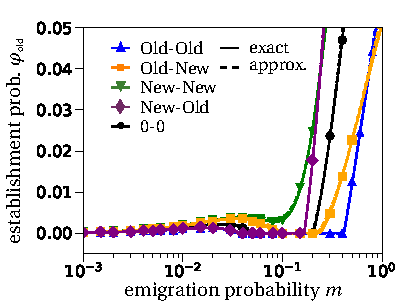
\includegraphics[width=\linewidth]{fig2a.pdf}
		\caption{$\omega^\text{old}_m=1.35$ (large fecundity difference)}
	\end{subfigure}%
	\begin{subfigure}{.5\textwidth}
		\centering
		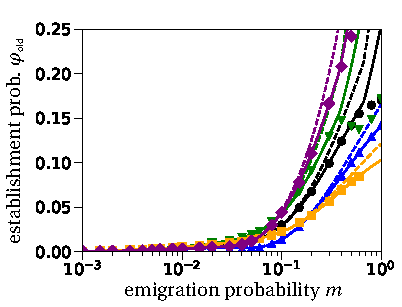
\includegraphics[width=\linewidth]{fig2c.pdf}
		\caption{$\omega^\text{old}_m=1.45$ (small fecundity difference)}
	\end{subfigure}
	\begin{subfigure}{.5\textwidth}
		\centering
		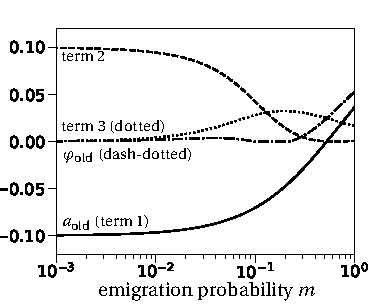
\includegraphics[width=\linewidth]{figS1c.pdf}
		\caption{$\omega^\text{old}_m=1.35$ (large fecundity difference)}
	\end{subfigure}%
	\begin{subfigure}{.5\textwidth}
		\centering
		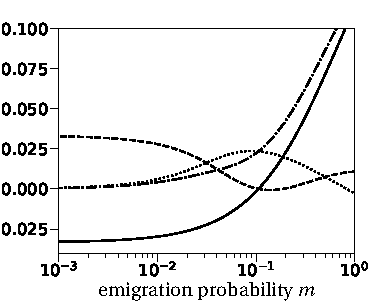
\includegraphics[width=\linewidth]{figS1d.pdf}
		\caption{$\omega^\text{old}_m=1.45$ (small fecundity difference)}
	\end{subfigure}
	\caption{\textbf{Contribution of the different terms in eq.~\eqref{Seq:estab_approx} to the establishment probability $\varphi_{\text{old}}$.} Subfigures (a,b) are the same as Figs.~\ref{fig:vary_m_est}(a,c) in the main text. They show the establishment probability for a single mutant individual arising in an old-habitat patch for varying emigration probabilities $m$. In subfigures (c,d) we plot the terms from eq.~\eqref{Seq:estab_approx} separately ($\pi_w=0.5,\pi_m=-0.5$). Term 1, the mutant growth rate in old habitats (solid), increases with increasing dispersal rates as a consequence of relaxed competition. Term 2, the environmental effect (dashed), captures the differences between the growth rates in the habitats. The larger the difference, the larger its contribution to the overall establishment probability. Term 3, the effect of dispersal (dotted), (largely) increases with increasing dispersal rates $m$. The sum of the three terms is plotted as a dash-dotted line.}
	\label{Sfig:contribution}
\end{figure}

For clarity, we re-plot Figs.~\ref{fig:vary_m_est}(a,c) in Fig.~\ref{Sfig:contribution}(a,b), respectively. We try to explain the ongoing processes for each of the regions through the approximations of the establishment probabilities in eq.~\eqref{Seq:estab_approx}, see also Fig.~\ref{Sfig:contribution}(c,d). Note that these explanations are only valid for the establishment probability of a mutant initially in an old-habitat patch, $\varphi_{\text{old}}$. For the intuition behind the shape of $\varphi_{\text{new}}$ we refer to the corresponding section in the main text.

Region (i) is explained by the positive effect of dispersal. Mutants disperse from old- to new-habitat patches where they \chg{have a higher growth rate}. This effect is mediated through the third term of the establishment probability in eq.~\eqref{Seq:estab_approx}. \chg{Note that the first two terms of the approximation cancel out for small emigration probabilities $m$.}
While the third term increases with increasing emigration rate $m$, the second term in eq.~\eqref{Seq:estab_approx} decreases, cf. Fig.~\ref{Sfig:contribution}. 
In the formula this is mediated through \chg{the increase of the local growth rate in the old-habitat, $a_{\text{old}}$, i.e.\ it becomes less negative. Then both factors of the second term, $a_{\text{old}}$ and the difference $(a_{\text{old}}-a_{\text{new}})$, increase (which in turn decreases term two). The }\chg{intuitive} reason is that due to larger emigration probabilities $m$, more individuals leave old habitats before the reproductive event. This relaxes competition in these patches and therefore increases the local growth rate of mutants in old-habitat patches.   
%
%The intuition is that habitat differences become less important under stronger population mixing -- recall that the dispersal rate $m$ appears in the constant $C$ in the denominator. This alone would explain the decreasing curve of the second term. Additionally though, the local growth rate in old-habitat patches, $a_{\text{old}}$, is linked to the population demography which changes for varying $m$. With larger dispersal rates, more individuals leave the densely populated old habitats. This results in alleviated competition pressure for the remaining individuals, thus increasing the local growth rate $a_{\text{old}}$. This decreases the difference of growth rates $a_{\text{old}}-a_{\text{new}}$. Therefore, the local maximum can be explained by the decreasing environmental influence and the increasing dispersal effect, the second and the third term in eq.~\eqref{eq:estab_approx}, respectively. Hence, region (ii), beginning with the local maximum, is dominated by the decreasing effect of the environment on the establishment probability. 
Finally, in region (iii) dispersal is so large that the population homogenizes. This results in even less competitive pressure in old-habitat patches. Eventually, this yields a positive growth rate $a_{\text{old}}$ (first term in eq.~\eqref{Seq:estab_approx}). Therefore, this region is driven by the local growth rate in old habitats.

Note that region (iii) can be shifted to the left by increasing the absolute number of offspring of mutants in old-habitat patches, $\omega^\text{old}_m$, and therefore decreasing the local disadvantage of the mutant. If shifted sufficiently to the left, like in Fig.~\ref{Sfig:contribution}(d), region (ii) might vanish due to this effect.

\chg{Contrarily, if we set the fecundity parameter of the mutant in the old habitat to $\omega^\text{old}_m=1.1$, we see that region (iii) disappears for most dispersal schemes, cf. Fig.~\ref{Sfig:weak_fecundity}. Due to the low fecundity of the mutant, even under relaxed competition in old habitats, establishment of a mutant population is very unlikely. The final increase of our approximation in the dispersal schemes New-New and New-Old is due to our density-independence assumption in new habitats. For these large values of $m$ and the bias of the wild type towards new-habitat patches, this assumption is violated in the simulations explaining the deviation from the simulation results and our prediction. }

\begin{figure}
	\centering
	\begin{subfigure}{.5\textwidth}
		\centering
		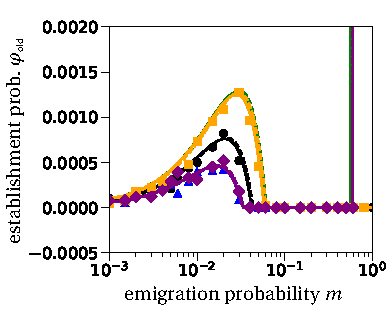
\includegraphics[width=\linewidth]{figS2a.pdf}
		\caption{$\varphi_{\text{old}}$}
	\end{subfigure}%
	\begin{subfigure}{.5\textwidth}
		\centering
		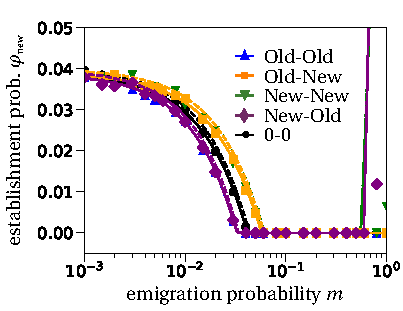
\includegraphics[width=\linewidth]{figS2b.pdf}
		\caption{$\varphi_{\text{new}}$}
	\end{subfigure}
	\caption{\textbf{Disappearance of region (iii) for large fecundity differences in the old habitat.} If the mutant fecundity in old-habitat patches is too low, here $\omega^\text{old}_m=1.1$, the effect of relaxed competition is not strong enough to have an impact on the establishment probability for high dispersal rates. The establishment probability remains at zero.}
	\label{Sfig:weak_fecundity}
\end{figure}


%%%%%%%%%%%%%%%%%%%%%%%%%%%%%%%%%%%%%%%%%%%%%%%%%%%%%%%%%
% Native habitat type %%%%%%%%%%%%%%%%%%%%%%%%%%%%%%%%%%%
%%%%%%%%%%%%%%%%%%%%%%%%%%%%%%%%%%%%%%%%%%%%%%%%%%%%%%%%%
\newpage
\renewcommand{\theequation}{C\arabic{equation}}
\setcounter{equation}{0}  % reset counter 

\section{Habitat of origin of the adaptive mutation}
\chg{Here, we provide further insight into the origin of the adaptive mutation. Therefore we plot the establishment probabilities $\varphi_{\text{old}}$ and $\varphi_{\text{new}}$ when varying the frequency of old habitats, $f_{\text{old}}$. In Fig.~\ref{fig:origin} in the main text we have seen that most successful adaptive mutations arise in old-habitat patches. Here, we show that this is explained mostly due to the large mutational input that is provided by the much larger wild-type population sizes in old habitats, see Fig.~\ref{Sfig:vary_f_origin}(b). The establishment probability though is always larger for mutants that arise in new habitats than in old habitats (Fig.~\ref{Sfig:vary_f_origin}(a)). 
}

\begin{figure}[h!]
	\centering
	\begin{subfigure}{.5\textwidth}
		\centering
		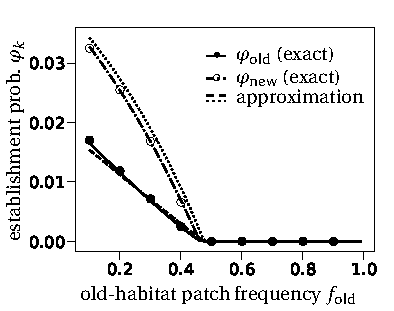
\includegraphics[width=\linewidth]{figS3a.pdf}
		\caption{Establishment probabilities}
	\end{subfigure}%
	\begin{subfigure}{.5\textwidth}
		\centering
		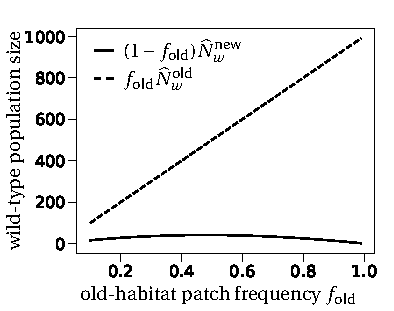
\includegraphics[width=\linewidth]{figS3b.pdf}
		\caption{Stationary wild-type population size}
	\end{subfigure}
	\caption{\textbf{Establishment probability and stationary wild-type population size when varying the old-habitat frequency.} In the simulations we have used the standard set of parameters as given in Table~\ref{tab:parameters} and the unbiased dispersal scheme ($\pi_w=\pi_m=0$). In (a) we additionally chose the large fecundity difference scenario ($\omega^\text{old}_m=1.35$).}
	\label{Sfig:vary_f_origin}
\end{figure}

%Additionally, we investigate the habitat type of the origin of the adaptive mutations for low fecundity values of the mutant in the old habitat. While for large fecundity values of the mutant in the old habitat most successful lineages arise in the old habitat (Fig.~\ref{fig:origin} in the main text), we see that for lower fecundity values $\omega^\text{old}_m$ the contribution of new-habitat mutants approaches and occasionally exceeds the number of successful mutant lineages that emerge from old-habitat patches. In the subsequent figure, besides the default parameters as stated in Table 1 in the main text, we chose $\omega^\text{old}_m=1.05$ and $\theta = 10/(MK)$. The plot corresponding to Fig.~\ref{fig:origin} in the main text then looks as follows:

%\begin{figure}[h!]
%	\centering
%	\includegraphics[width=0.6\textwidth]{figS4.pdf}
%  	\caption{\textbf{Habitat type of the origin for strong fecundity differences in the old habitat ($\omega^\text{old}_m=1.05$).}}
%	\label{Sfig:origin}
%\end{figure}
\pete{There was a figure where the contribution from new habitats was larger than from old habitats. With the changed fecundities, I only get this behavior if the fecundity of the mutant is larger in the new patches than in the old patches, i.e. $\omega^\text{old}_m < a_{\text{new}}$. Also, for some reason the approximations do not work that well in these scenarios (I did not investigate why the estimated lines are bad -- soft sweeps still work fine but the other approximations don't.)}

%%%%%%%%%%%%%%%%%%%%%%%%%%%%%%%%%%%%%%%%%%%%%%%%%%%%%%%%%
% Large emigration rate %%%%%%%%%%%%%%%%%%%%%%%%%%%%%%%%%
%%%%%%%%%%%%%%%%%%%%%%%%%%%%%%%%%%%%%%%%%%%%%%%%%%%%%%%%%
\newpage
\renewcommand{\theequation}{D\arabic{equation}}
\setcounter{equation}{0}  % reset counter 

\section{Probability of establishment for large frequencies of old-habitat patches}
\chg{We plot the probability of establishment for a large frequency of old-habitat patches, $f_{\text{old}}$. As visible in Fig.~\ref{Sfig:vary_f} below, for high frequencies of old-habitat patches the probability of adaptation becomes very small, if not zero, for large emigration probabilities $m$. These high frequency of old-habitat patches are the patch configurations which mutants that were present before the first patch degrades, i.e. standing genetic variation mutants, experience. Therefore, it is very unlikely that the mutant, which will eventually rescue the population, was already present before the first degradation event.} This supports the explanation that homogenizing the population (large $m$) reduces the impact of standing genetic variation on the probability of evolutionary rescue, see Fig.~\ref{fig:sgv}(b) in the main text where $\pi_w=\pi_m=0$ was plotted.

\begin{figure}[h!]
	\centering
	\begin{subfigure}{.5\textwidth}
		\centering
		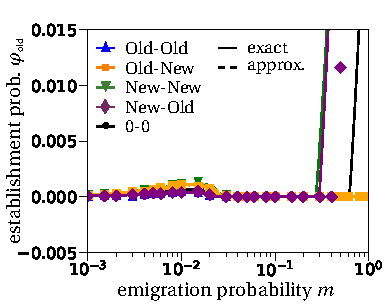
\includegraphics[width=\linewidth]{figS5a.pdf}
		\caption{$\varphi_{\text{old}}$}
	\end{subfigure}%
	\begin{subfigure}{.5\textwidth}
		\centering
		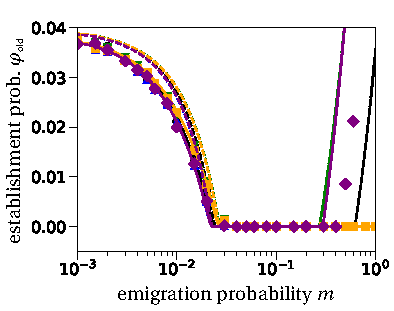
\includegraphics[width=\linewidth]{figS5b.pdf}
		\caption{$\varphi_{\text{new}}$}
	\end{subfigure}
	\caption{\textbf{Probability of adaptation for a large frequency of old-habitat patches ($f_{\text{old}}=0.9$).} The fecundity of the mutant in old-habitat patches is set to $\omega^\text{old}_m=1.45$. Note also the difference between the scales of the y-axes in the two panels.}
	\label{Sfig:vary_f}
\end{figure}

%%%%%%%%%%%%%%%%%%%%%%%%%%%%%%%%%%%%%%%%%%%%%%%%%%%%%%%%%
% Comparison to pop gen %%%%%%%%%%%%%%%%%%%%%%%%%%%%%%%%%
%%%%%%%%%%%%%%%%%%%%%%%%%%%%%%%%%%%%%%%%%%%%%%%%%%%%%%%%%
\newpage
\renewcommand{\theequation}{E\arabic{equation}}
\setcounter{equation}{0}  % reset counter 

\section{Establishment probability in a model without demography}
Here, we consider a variation of our original model in order to investigate the impact of demography on the establishment probabilities $\varphi_{\text{old}}$ and $\varphi_{\text{new}}$. The dispersal process and the dynamics in old-habitat patches remain as studied before. In new-habitat patches we now assume that the population remains at carrying capacity, i.e. there is no longer a declining wild-type population. This means that the local growth rate $a_{\text{old}}$ in eq.~\eqref{Seq:s_old} takes the form for $\widehat{N}_w^{\text{new}}=K_{\text{new}}$. For simplicity we will also assume that $K_{\text{new}}=K_{\text{old}}=K$. In order to maintain the divergent selection assumption, we assume that the fecundity of the wild-type in the new habitat is below the fecundity of the mutant. %For simplicity, we assume that the fecundity values are given as
%\begin{equation}
%    \omega^\text{old}_w^{\text{old}} = \omega^\text{old}_m^{\text{new}} \quad \text{and} \quad \omega^\text{old}_w^{\text{new}} = \omega^\text{old}_m^{\text{old}}.
%\end{equation}
Therefore, we need to adjust the local growth rate of a single mutant, $a_{\text{new}}$. The local growth rate in old habitats, $a_{\text{old}}$, remains as outlined in eq.~\eqref{Seq:s_old}. We have
\begin{equation}
1+a_{\text{new}} = K \frac{\omega_m^{\text{new}}}{\omega_w^{\text{new}} \widetilde{N}_w^{\text{new}}+ \omega_m^{\text{new}}}\approx K \frac{\omega_m^{\text{new}}}{\omega_w^{\text{new}} \widetilde{N}_w^{\text{new}}},
\end{equation}
which with the help of eq.~\eqref{Seq:wt_eq1} yields
\begin{equation}
a_{\text{new}} \approx \frac{\omega_m^{\text{new}}}{\omega_w^{\text{new}}\left(1+\frac{m f_{\text{old}} (1-\widehat{\pi}_w)}{1-f_{\text{old}}+\widehat{\pi}_w f_{\text{old}}}\right)}.
\end{equation}

\chg{Note, that we again used that during the establishment phase the wild type is much more abundant than the mutant which explains the approximation in the two equations.}
Plugging this in the approximation of the establishment probability from eq.~\eqref{Seq:estab_approx} we find the curves in Fig.~\ref{Sfig:pop_gen}.

We see that, as briefly mentioned in the main text, region (iii) of the establishment probability disappears in these type of models except for the Old-New and the New-Old dispersal schemes. The reason for the disappearance of the region is that relaxed competition only plays a subordinate role for the symmetric dispersal schemes (Old-Old, New-New and 0-0). In other words, these dispersal schemes maintain the local frequencies of the mutant at the same level as before the dispersal step and by that do not change the population dynamics. In contrast, the Old-New dispersal scheme strongly increases the frequency of mutants in new-habitat patches and by that increases the establishment probability. It is worth mentioning though, that this is not an effect of relaxed competition but rather a biased dispersal of the mutant into the habitat where it is favored. Solely for the New-Old dispersal scheme where individuals prefer the habitat they are relatively less fit, we see a relaxed competition scenario in old-habitat patches. For high dispersal rates $m$ the majority of the wild-type individuals emigrate to new habitats and by that leave space for the rare mutants in old-habitat patches to reproduce. This explains why this dispersal scheme still shows the characteristic pattern of a three-stage establishment probability.   \newpage 

\begin{figure}[h!]
	\centering
	\begin{subfigure}{.5\textwidth}
		\centering
		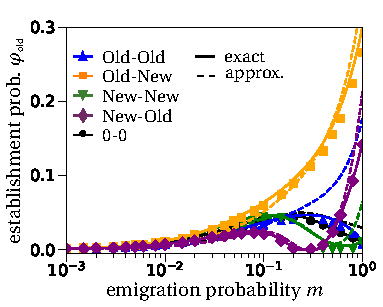
\includegraphics[width=\linewidth]{figS6a.pdf}
		\caption{$\varphi_{\text{old}}$ with $\omega^\text{old}_m=1.35$ (large fecundity difference)}
	\end{subfigure}%
	\begin{subfigure}{.5\textwidth}
		\centering
		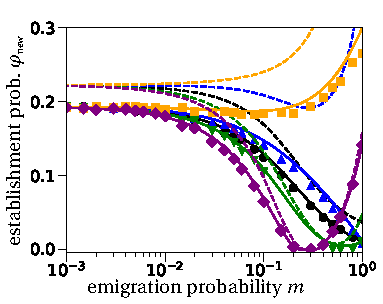
\includegraphics[width=\linewidth]{figS6b.pdf}
		\caption{$\varphi_{\text{new}}$ with $\omega^\text{old}_m=1.35$}
	\end{subfigure}
	\begin{subfigure}{.5\textwidth}
		\centering
		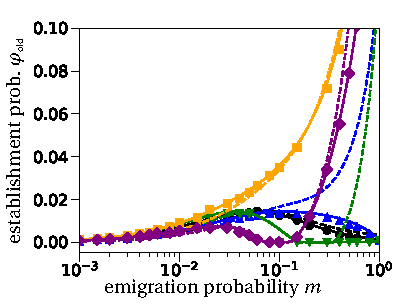
\includegraphics[width=\linewidth]{figS6c.pdf}
		\caption{$\varphi_{\text{old}}$ with $\omega^\text{old}_m=1.45$ (small fecundity difference)}
	\end{subfigure}%
	\begin{subfigure}{.5\textwidth}
		\centering
		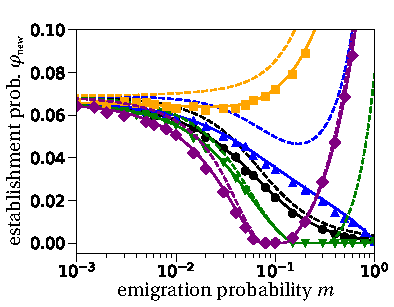
\includegraphics[width=\linewidth]{figS6d.pdf}
		\caption{$\varphi_{\text{new}}$ with $\omega^\text{old}_m=1.45$}
	\end{subfigure}
	\caption{\textbf{Establishment probability when populations in both habitats are at carrying capacity.} We plot the establishment probability for a single mutant either initially in an old-habitat patch (a,c) or in a new-habitat patch (b,d). The numerical solution (solid lines) still approximates the simulated data reasonably well. The analytical approximation (dashed lines) however deviates strongly from the data due to large growth rates ($a_{\text{new}}\approx 0.2$) so that the conditions for the approximation to hold are violated. In this case, in eq.~\eqref{Seq:estab_approx} higher order corrections would need to be taken into account. \chg{The fecundity values in the new habitat are given by $\omega_w^{\text{new}} = \omega_m^{\text{old}}$ and $\omega_m^{\text{new}} = \omega_w^{\text{old}}$ and the carrying capacity is $K_{\text{new}}=K_{\text{old}}=K=500$.} Missing data points (mostly for the negative density-dependent dispersal scheme -- green triangles) are explained by too large computation times. All data points are averages from $10^4$ independent runs. Note the varying y-axes scales.}
	\label{Sfig:pop_gen}
\end{figure}


%%%%%%%%%%%%%%%%%%%%%%%%%%%%%%%%%%%%%%%%%%%%%%%%%%%%%%%%%
% Origin dispersal schemes %%%%%%%%%%%%%%%%%%%%%%%%%%%%%%
%%%%%%%%%%%%%%%%%%%%%%%%%%%%%%%%%%%%%%%%%%%%%%%%%%%%%%%%%
\newpage
\renewcommand{\theequation}{F\arabic{equation}}
\setcounter{equation}{0}  % reset counter 
\section{Habitat of origin dependent on the dispersal scheme}
The habitat type of the origin of the rescue mutation is largely independent of the considered dispersal scheme. For $\omega^\text{old}_m=1.35$ we have plotted the relative contribution of each natal habitat type to the probability of evolutionary rescue, Fig.~\ref{Sfig:natal_habitat}. We do not see large differences between the three symmetric dispersal schemes (0-0, Old-Old, and New-New) and the Old-New dispersal scheme. \chg{Only for the New-Old dispersal schemes we see an increase in the contribution of mutants emerging from old-habitat patches for very high emigration probabilities $m$. A possible explanation is the large probability of establishment for a mutant emerging in old-habitat patches for this parameter set (cf. Fig.~\ref{Sfig:contribution}(a)).}

\begin{figure}[h!]
	\centering
	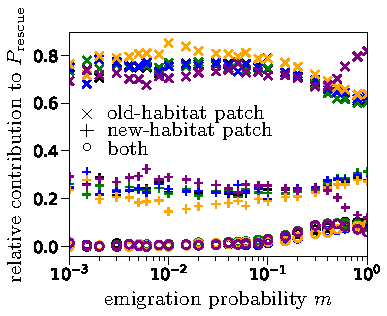
\includegraphics[width=0.6\textwidth]{figS7.pdf}
	\caption{\textbf{Habitat type of the origin of the rescue mutant dependent on the dispersal scheme.} Varying the emigration probability $m$ we plot the relative contributions of each habitat type to the probability of evolutionary rescue. The color-coding is as in the main text: black for 0-0, blue for the Old-Old, green for the New-New, orange for the Old-New, and purple for the New-Old dispersal scheme.}
	\label{Sfig:natal_habitat}
\end{figure}

%%%%%%%%%%%%%%%%%%%%%%%%%%%%%%%%%%%%%%%%%%%%%%%%%%%%%%%%%
% Bibliography %%%%%%%%%%%%%%%%%%%%%%%%%%%%%%%%%%%%%%%%%%
%%%%%%%%%%%%%%%%%%%%%%%%%%%%%%%%%%%%%%%%%%%%%%%%%%%%%%%%%
%\newpage
%\bibliographystyle{plainnat}
%\bibliography{dispersal.bib}


\end{document}